% Options for packages loaded elsewhere
\PassOptionsToPackage{unicode}{hyperref}
\PassOptionsToPackage{hyphens}{url}
%
\documentclass[
  11pt,
]{article}
\usepackage{lmodern}
\usepackage{amssymb,amsmath}
\usepackage{ifxetex,ifluatex}
\ifnum 0\ifxetex 1\fi\ifluatex 1\fi=0 % if pdftex
  \usepackage[T1]{fontenc}
  \usepackage[utf8]{inputenc}
  \usepackage{textcomp} % provide euro and other symbols
\else % if luatex or xetex
  \usepackage{unicode-math}
  \defaultfontfeatures{Scale=MatchLowercase}
  \defaultfontfeatures[\rmfamily]{Ligatures=TeX,Scale=1}
\fi
% Use upquote if available, for straight quotes in verbatim environments
\IfFileExists{upquote.sty}{\usepackage{upquote}}{}
\IfFileExists{microtype.sty}{% use microtype if available
  \usepackage[]{microtype}
  \UseMicrotypeSet[protrusion]{basicmath} % disable protrusion for tt fonts
}{}
\makeatletter
\@ifundefined{KOMAClassName}{% if non-KOMA class
  \IfFileExists{parskip.sty}{%
    \usepackage{parskip}
  }{% else
    \setlength{\parindent}{0pt}
    \setlength{\parskip}{6pt plus 2pt minus 1pt}}
}{% if KOMA class
  \KOMAoptions{parskip=half}}
\makeatother
\usepackage{xcolor}
\IfFileExists{xurl.sty}{\usepackage{xurl}}{} % add URL line breaks if available
\IfFileExists{bookmark.sty}{\usepackage{bookmark}}{\usepackage{hyperref}}
\hypersetup{
  pdftitle={Series Temporales - Trabajo Final},
  pdfauthor={Esteban Schab - Anabella De Battista},
  hidelinks,
  pdfcreator={LaTeX via pandoc}}
\urlstyle{same} % disable monospaced font for URLs
\usepackage[margin=1in]{geometry}
\usepackage{color}
\usepackage{fancyvrb}
\newcommand{\VerbBar}{|}
\newcommand{\VERB}{\Verb[commandchars=\\\{\}]}
\DefineVerbatimEnvironment{Highlighting}{Verbatim}{commandchars=\\\{\}}
% Add ',fontsize=\small' for more characters per line
\usepackage{framed}
\definecolor{shadecolor}{RGB}{248,248,248}
\newenvironment{Shaded}{\begin{snugshade}}{\end{snugshade}}
\newcommand{\AlertTok}[1]{\textcolor[rgb]{0.94,0.16,0.16}{#1}}
\newcommand{\AnnotationTok}[1]{\textcolor[rgb]{0.56,0.35,0.01}{\textbf{\textit{#1}}}}
\newcommand{\AttributeTok}[1]{\textcolor[rgb]{0.77,0.63,0.00}{#1}}
\newcommand{\BaseNTok}[1]{\textcolor[rgb]{0.00,0.00,0.81}{#1}}
\newcommand{\BuiltInTok}[1]{#1}
\newcommand{\CharTok}[1]{\textcolor[rgb]{0.31,0.60,0.02}{#1}}
\newcommand{\CommentTok}[1]{\textcolor[rgb]{0.56,0.35,0.01}{\textit{#1}}}
\newcommand{\CommentVarTok}[1]{\textcolor[rgb]{0.56,0.35,0.01}{\textbf{\textit{#1}}}}
\newcommand{\ConstantTok}[1]{\textcolor[rgb]{0.00,0.00,0.00}{#1}}
\newcommand{\ControlFlowTok}[1]{\textcolor[rgb]{0.13,0.29,0.53}{\textbf{#1}}}
\newcommand{\DataTypeTok}[1]{\textcolor[rgb]{0.13,0.29,0.53}{#1}}
\newcommand{\DecValTok}[1]{\textcolor[rgb]{0.00,0.00,0.81}{#1}}
\newcommand{\DocumentationTok}[1]{\textcolor[rgb]{0.56,0.35,0.01}{\textbf{\textit{#1}}}}
\newcommand{\ErrorTok}[1]{\textcolor[rgb]{0.64,0.00,0.00}{\textbf{#1}}}
\newcommand{\ExtensionTok}[1]{#1}
\newcommand{\FloatTok}[1]{\textcolor[rgb]{0.00,0.00,0.81}{#1}}
\newcommand{\FunctionTok}[1]{\textcolor[rgb]{0.00,0.00,0.00}{#1}}
\newcommand{\ImportTok}[1]{#1}
\newcommand{\InformationTok}[1]{\textcolor[rgb]{0.56,0.35,0.01}{\textbf{\textit{#1}}}}
\newcommand{\KeywordTok}[1]{\textcolor[rgb]{0.13,0.29,0.53}{\textbf{#1}}}
\newcommand{\NormalTok}[1]{#1}
\newcommand{\OperatorTok}[1]{\textcolor[rgb]{0.81,0.36,0.00}{\textbf{#1}}}
\newcommand{\OtherTok}[1]{\textcolor[rgb]{0.56,0.35,0.01}{#1}}
\newcommand{\PreprocessorTok}[1]{\textcolor[rgb]{0.56,0.35,0.01}{\textit{#1}}}
\newcommand{\RegionMarkerTok}[1]{#1}
\newcommand{\SpecialCharTok}[1]{\textcolor[rgb]{0.00,0.00,0.00}{#1}}
\newcommand{\SpecialStringTok}[1]{\textcolor[rgb]{0.31,0.60,0.02}{#1}}
\newcommand{\StringTok}[1]{\textcolor[rgb]{0.31,0.60,0.02}{#1}}
\newcommand{\VariableTok}[1]{\textcolor[rgb]{0.00,0.00,0.00}{#1}}
\newcommand{\VerbatimStringTok}[1]{\textcolor[rgb]{0.31,0.60,0.02}{#1}}
\newcommand{\WarningTok}[1]{\textcolor[rgb]{0.56,0.35,0.01}{\textbf{\textit{#1}}}}
\usepackage{graphicx,grffile}
\makeatletter
\def\maxwidth{\ifdim\Gin@nat@width>\linewidth\linewidth\else\Gin@nat@width\fi}
\def\maxheight{\ifdim\Gin@nat@height>\textheight\textheight\else\Gin@nat@height\fi}
\makeatother
% Scale images if necessary, so that they will not overflow the page
% margins by default, and it is still possible to overwrite the defaults
% using explicit options in \includegraphics[width, height, ...]{}
\setkeys{Gin}{width=\maxwidth,height=\maxheight,keepaspectratio}
% Set default figure placement to htbp
\makeatletter
\def\fps@figure{htbp}
\makeatother
\setlength{\emergencystretch}{3em} % prevent overfull lines
\providecommand{\tightlist}{%
  \setlength{\itemsep}{0pt}\setlength{\parskip}{0pt}}
\setcounter{secnumdepth}{-\maxdimen} % remove section numbering
\usepackage{booktabs}
\usepackage{booktabs}
\usepackage{longtable}
\usepackage{array}
\usepackage{multirow}
\usepackage{wrapfig}
\usepackage{float}
\usepackage{colortbl}
\usepackage{pdflscape}
\usepackage{tabu}
\usepackage{threeparttable}
\usepackage{threeparttablex}
\usepackage[normalem]{ulem}
\usepackage{makecell}
\usepackage{xcolor}

\title{Series Temporales - Trabajo Final}
\author{Esteban Schab - Anabella De Battista}
\date{Febrero 2021}

\begin{document}
\maketitle

{
\setcounter{tocdepth}{2}
\tableofcontents
}
\begin{Shaded}
\begin{Highlighting}[]
\NormalTok{archivo <-}\StringTok{ './data/Datos-dax-nasdaq-originales.xlsx'}
\NormalTok{dax_nasdaq_dow <-}\StringTok{ }\KeywordTok{read_excel}\NormalTok{(archivo, }\DataTypeTok{col_names =} \OtherTok{TRUE}\NormalTok{)}
\KeywordTok{names}\NormalTok{(dax_nasdaq_dow)}
\end{Highlighting}
\end{Shaded}

\begin{verbatim}
## [1] "Fecha"                            "DAX 30 PERFORMANCE - PRICE INDEX"
## [3] "NASDAQ COMPOSITE - PRICE INDEX"
\end{verbatim}

\begin{Shaded}
\begin{Highlighting}[]
\KeywordTok{names}\NormalTok{(dax_nasdaq_dow) <-}\StringTok{ }\KeywordTok{c}\NormalTok{(}\StringTok{"Fecha"}\NormalTok{, }\StringTok{"DAX"}\NormalTok{, }\StringTok{"NASDAQ"}\NormalTok{)}
\KeywordTok{names}\NormalTok{(dax_nasdaq_dow)}
\end{Highlighting}
\end{Shaded}

\begin{verbatim}
## [1] "Fecha"  "DAX"    "NASDAQ"
\end{verbatim}

\begin{Shaded}
\begin{Highlighting}[]
\KeywordTok{summary}\NormalTok{(dax_nasdaq_dow)}
\end{Highlighting}
\end{Shaded}

\begin{verbatim}
##      Fecha                          DAX              NASDAQ        
##  Min.   :1971-02-05 00:00:00   Min.   :  372.3   Min.   :   54.87  
##  1st Qu.:1983-07-21 18:00:00   1st Qu.:  710.9   1st Qu.:  247.13  
##  Median :1996-01-04 12:00:00   Median : 2320.2   Median : 1057.44  
##  Mean   :1996-01-05 02:24:00   Mean   : 4048.6   Mean   : 1877.67  
##  3rd Qu.:2008-06-19 06:00:00   3rd Qu.: 6351.3   3rd Qu.: 2508.07  
##  Max.   :2020-12-03 00:00:00   Max.   :13789.0   Max.   :12377.18
\end{verbatim}

\begin{Shaded}
\begin{Highlighting}[]
\NormalTok{indice_dax <-}\StringTok{ }\KeywordTok{as.numeric}\NormalTok{(}\KeywordTok{unlist}\NormalTok{(dax_nasdaq_dow[,}\StringTok{"DAX"}\NormalTok{]))}
\NormalTok{rend_log_dax <-}\StringTok{ }\KeywordTok{diff}\NormalTok{(}\KeywordTok{log}\NormalTok{(indice_dax))}
\CommentTok{#agrego un 0 al principio para poder agregar la columna de rendimientos al dataframe original }
\NormalTok{rend_log_dax <-}\StringTok{ }\KeywordTok{c}\NormalTok{(}\DecValTok{0}\NormalTok{, rend_log_dax)}

\NormalTok{indice_nasdaq <-}\StringTok{ }\KeywordTok{as.numeric}\NormalTok{(}\KeywordTok{unlist}\NormalTok{(dax_nasdaq_dow[,}\StringTok{"NASDAQ"}\NormalTok{]))}
\NormalTok{rend_log_nasdaq <-}\StringTok{ }\KeywordTok{diff}\NormalTok{(}\KeywordTok{log}\NormalTok{(indice_nasdaq))}
\CommentTok{#agrego un NA al principio para poder agregar la columna de rendimientos al dataframe original }
\NormalTok{rend_log_nasdaq <-}\StringTok{ }\KeywordTok{c}\NormalTok{(}\DecValTok{0}\NormalTok{, rend_log_nasdaq)}
\end{Highlighting}
\end{Shaded}

\begin{Shaded}
\begin{Highlighting}[]
\NormalTok{df_dax_nasdaq_dow <-}\StringTok{ }\KeywordTok{cbind}\NormalTok{(dax_nasdaq_dow,}
                           \DataTypeTok{rdto_dax=}\NormalTok{rend_log_dax, }
                           \DataTypeTok{rdto_nasdaq=}\NormalTok{rend_log_nasdaq}
\NormalTok{                           )}

\CommentTok{# reordenamos columnas}
\NormalTok{df_dax_nasdaq_dow <-}\StringTok{ }\NormalTok{df_dax_nasdaq_dow[, }\KeywordTok{c}\NormalTok{(}\DecValTok{1}\NormalTok{, }\DecValTok{2}\NormalTok{, }\DecValTok{4}\NormalTok{, }\DecValTok{3}\NormalTok{, }\DecValTok{5}\NormalTok{)]}
\KeywordTok{head}\NormalTok{(df_dax_nasdaq_dow)}
\end{Highlighting}
\end{Shaded}

\begin{verbatim}
##        Fecha    DAX     rdto_dax NASDAQ   rdto_nasdaq
## 1 1971-02-05 508.42  0.000000000 100.00  0.0000000000
## 2 1971-02-08 509.65  0.002416338 100.84  0.0083649163
## 3 1971-02-09 506.30 -0.006594837 100.76 -0.0007936508
## 4 1971-02-10 501.95 -0.008628866 100.69 -0.0006949616
## 5 1971-02-11 503.89  0.003857477 101.45  0.0075195763
## 6 1971-02-12 513.04  0.017995825 102.05  0.0058968230
\end{verbatim}

Se muestran las estadísticas principales del dataset.

\begin{Shaded}
\begin{Highlighting}[]
\KeywordTok{summary}\NormalTok{(df_dax_nasdaq_dow)}
\end{Highlighting}
\end{Shaded}

\begin{verbatim}
##      Fecha                          DAX             rdto_dax         
##  Min.   :1971-02-05 00:00:00   Min.   :  372.3   Min.   :-0.1370990  
##  1st Qu.:1983-07-21 18:00:00   1st Qu.:  710.9   1st Qu.:-0.0055691  
##  Median :1996-01-04 12:00:00   Median : 2320.2   Median : 0.0002207  
##  Mean   :1996-01-05 02:24:00   Mean   : 4048.6   Mean   : 0.0002508  
##  3rd Qu.:2008-06-19 06:00:00   3rd Qu.: 6351.3   3rd Qu.: 0.0065904  
##  Max.   :2020-12-03 00:00:00   Max.   :13789.0   Max.   : 0.1079747  
##      NASDAQ          rdto_nasdaq        
##  Min.   :   54.87   Min.   :-0.1314915  
##  1st Qu.:  247.13   1st Qu.:-0.0041536  
##  Median : 1057.44   Median : 0.0007315  
##  Mean   : 1877.67   Mean   : 0.0003706  
##  3rd Qu.: 2508.07   3rd Qu.: 0.0058327  
##  Max.   :12377.18   Max.   : 0.1325465
\end{verbatim}

Estadísticas más completas del rendimiento del índice dax

\begin{Shaded}
\begin{Highlighting}[]
\CommentTok{#Cálculo simple de estadíticos descriptivos}
\NormalTok{min <-}\StringTok{ }\KeywordTok{min}\NormalTok{(df_dax_nasdaq_dow}\OperatorTok{$}\NormalTok{rdto_dax, }\DataTypeTok{na.rm =} \OtherTok{TRUE}\NormalTok{)}
\NormalTok{q1 <-}\StringTok{ }\KeywordTok{quantile}\NormalTok{(df_dax_nasdaq_dow}\OperatorTok{$}\NormalTok{rdto_dax, }\DataTypeTok{probs =} \FloatTok{0.25}\NormalTok{, }\DataTypeTok{na.rm =} \OtherTok{TRUE}\NormalTok{)}
\NormalTok{media <-}\StringTok{ }\KeywordTok{mean.default}\NormalTok{(df_dax_nasdaq_dow}\OperatorTok{$}\NormalTok{rdto_dax, }\DataTypeTok{na.rm =} \OtherTok{TRUE}\NormalTok{)}
\NormalTok{media_rec <-}\StringTok{ }\KeywordTok{mean.default}\NormalTok{(df_dax_nasdaq_dow}\OperatorTok{$}\NormalTok{rdto_dax, }\DataTypeTok{trim =} \FloatTok{0.025}\NormalTok{, }\DataTypeTok{na.rm =} \OtherTok{TRUE}\NormalTok{)}
\NormalTok{mediana <-}\StringTok{ }\KeywordTok{median.default}\NormalTok{(df_dax_nasdaq_dow}\OperatorTok{$}\NormalTok{rdto_dax, }\DataTypeTok{na.rm =} \OtherTok{TRUE}\NormalTok{)}
\NormalTok{moda <-}\StringTok{ }\KeywordTok{mfv}\NormalTok{(df_dax_nasdaq_dow}\OperatorTok{$}\NormalTok{rdto_dax)}
\NormalTok{var <-}\StringTok{ }\KeywordTok{var}\NormalTok{(df_dax_nasdaq_dow}\OperatorTok{$}\NormalTok{rdto_dax, }\DataTypeTok{na.rm =} \OtherTok{TRUE}\NormalTok{)}
\NormalTok{desvest <-}\StringTok{ }\KeywordTok{sd}\NormalTok{(df_dax_nasdaq_dow}\OperatorTok{$}\NormalTok{rdto_dax, }\DataTypeTok{na.rm =} \OtherTok{TRUE}\NormalTok{)}
\NormalTok{q3 <-}\StringTok{ }\KeywordTok{quantile}\NormalTok{(df_dax_nasdaq_dow}\OperatorTok{$}\NormalTok{rdto_dax, }\DataTypeTok{probs =} \FloatTok{0.75}\NormalTok{, }\DataTypeTok{na.rm =} \OtherTok{TRUE}\NormalTok{)}
\NormalTok{max <-}\StringTok{ }\KeywordTok{max}\NormalTok{(df_dax_nasdaq_dow}\OperatorTok{$}\NormalTok{rdto_dax, }\DataTypeTok{na.rm =} \OtherTok{TRUE}\NormalTok{)}
\NormalTok{s <-}\StringTok{ }\KeywordTok{skew}\NormalTok{(df_dax_nasdaq_dow}\OperatorTok{$}\NormalTok{rdto_dax)}
\NormalTok{c <-}\StringTok{ }\KeywordTok{kurtosi}\NormalTok{(df_dax_nasdaq_dow}\OperatorTok{$}\NormalTok{rdto_dax)}

\CommentTok{#Valores de estadísticos como vector}
\NormalTok{descriptivos_rdto_dax <-}\StringTok{ }\KeywordTok{as.numeric}\NormalTok{(}\KeywordTok{round}\NormalTok{(}\KeywordTok{c}\NormalTok{(min, q1, media, media_rec, mediana, moda,}
\NormalTok{                          var, desvest, q3, max, s, c),}\DecValTok{5}\NormalTok{))}

\NormalTok{nombres_desc_rdto_dax <-}\StringTok{ }\KeywordTok{c}\NormalTok{(}\StringTok{"Mínimo"}\NormalTok{, }\StringTok{"Q1"}\NormalTok{, }\StringTok{"Media"}\NormalTok{, }\StringTok{"Media recortada"}\NormalTok{, }\StringTok{"Mediana"}\NormalTok{, }\StringTok{"Moda"}\NormalTok{,}
             \StringTok{"Varianza"}\NormalTok{, }\StringTok{"Desviación Estándar"}\NormalTok{, }\StringTok{"Q3"}\NormalTok{, }\StringTok{"Máximo"}\NormalTok{, }\StringTok{"Simetría"}\NormalTok{, }\StringTok{"Curtosis"}\NormalTok{)}

\NormalTok{cuadro_eda_dax <-}\StringTok{ }\KeywordTok{as.data.frame}\NormalTok{(}\KeywordTok{rbind}\NormalTok{(nombres_desc_rdto_dax,descriptivos_rdto_dax))}
\NormalTok{tabla_eda_dax <-}\StringTok{ }\KeywordTok{data.frame}\NormalTok{(}\KeywordTok{t}\NormalTok{(cuadro_eda_dax[}\OperatorTok{-}\DecValTok{1}\NormalTok{]),}\DataTypeTok{row.names =} \OtherTok{NULL}\NormalTok{)}
\KeywordTok{colnames}\NormalTok{(tabla_eda_dax) <-}\StringTok{ }\KeywordTok{c}\NormalTok{(}\StringTok{"Estadístico"}\NormalTok{,}\StringTok{"rdto_dax"}\NormalTok{)}
\CommentTok{#tabla_eda_dax}
\end{Highlighting}
\end{Shaded}

\begin{Shaded}
\begin{Highlighting}[]
\CommentTok{# Generación de una tabla}
\KeywordTok{kable}\NormalTok{(tabla_eda_dax, }\DataTypeTok{align =} \KeywordTok{c}\NormalTok{(}\StringTok{"l"}\NormalTok{, }\StringTok{"c"}\NormalTok{)) }\OperatorTok\StringTok{ }
\StringTok{  }\KeywordTok{kable_styling}\NormalTok{(}\DataTypeTok{full_width =}\NormalTok{ F, }\DataTypeTok{bootstrap_options =} \StringTok{"condensed"}\NormalTok{) }\OperatorTok\StringTok{ }
\StringTok{  }\KeywordTok{column_spec}\NormalTok{(}\DecValTok{1}\NormalTok{, }\DataTypeTok{width =} \StringTok{"12em"}\NormalTok{) }\OperatorTok\StringTok{ }
\StringTok{  }\KeywordTok{column_spec}\NormalTok{(}\DecValTok{2}\NormalTok{, }\DataTypeTok{width =} \StringTok{"10em"}\NormalTok{) }
\end{Highlighting}
\end{Shaded}

\begin{table}[H]
\centering
\begin{tabular}{>{\raggedright\arraybackslash}p{12em}|>{\centering\arraybackslash}p{10em}}
\hline
Estadístico & rdto\_dax\\
\hline
Q1 & -0.00557\\
\hline
Media & 0.00025\\
\hline
Media recortada & 0.00036\\
\hline
Mediana & 0.00022\\
\hline
Moda & 0\\
\hline
Varianza & 0.00016\\
\hline
Desviación Estándar & 0.01258\\
\hline
Q3 & 0.00659\\
\hline
Máximo & 0.10797\\
\hline
Simetría & -0.36556\\
\hline
Curtosis & 8.13234\\
\hline
\end{tabular}
\end{table}

Se agregan las columnas correspondientes a los días de la semana.

\begin{Shaded}
\begin{Highlighting}[]
\NormalTok{df_dax_nasdaq_dow <-}\StringTok{ }\KeywordTok{as_tibble}\NormalTok{(df_dax_nasdaq_dow)}
\NormalTok{df_dax_nasdaq_dow <-}\StringTok{ }\KeywordTok{mutate}\NormalTok{(df_dax_nasdaq_dow,}
                            \DataTypeTok{dia =} \KeywordTok{weekdays}\NormalTok{(df_dax_nasdaq_dow}\OperatorTok{$}\NormalTok{Fecha, }\DataTypeTok{abbreviate =} \OtherTok{FALSE}\NormalTok{)}
\NormalTok{)}
\NormalTok{df_dax_nasdaq_dow}\OperatorTok{$}\NormalTok{dia[df_dax_nasdaq_dow}\OperatorTok{$}\NormalTok{dia }\OperatorTok{==}\StringTok{ "miércoles"}\NormalTok{] <-}\StringTok{ "miercoles"}
\KeywordTok{head}\NormalTok{(df_dax_nasdaq_dow)}
\end{Highlighting}
\end{Shaded}

\begin{verbatim}
## # A tibble: 6 x 6
##   Fecha                 DAX rdto_dax NASDAQ rdto_nasdaq dia      
##   <dttm>              <dbl>    <dbl>  <dbl>       <dbl> <chr>    
## 1 1971-02-05 00:00:00  508.  0         100     0        viernes  
## 2 1971-02-08 00:00:00  510.  0.00242   101.    0.00836  lunes    
## 3 1971-02-09 00:00:00  506. -0.00659   101.   -0.000794 martes   
## 4 1971-02-10 00:00:00  502. -0.00863   101.   -0.000695 miercoles
## 5 1971-02-11 00:00:00  504.  0.00386   101.    0.00752  jueves   
## 6 1971-02-12 00:00:00  513.  0.0180    102.    0.00590  viernes
\end{verbatim}

\hypertarget{gruxe1fico-de-la-serie-temporal-de-rendimientos-del-uxedndice-dax}{%
\subsection{Gráfico de la serie temporal de rendimientos del índice
DAX}\label{gruxe1fico-de-la-serie-temporal-de-rendimientos-del-uxedndice-dax}}

\hypertarget{htmlwidget-683dc24e847baa9d2feb}{}

Se ordenan los días de la semana.

\begin{verbatim}
## [1] "viernes"   "lunes"     "martes"    "miercoles" "jueves"
\end{verbatim}

\begin{verbatim}
## [1] "lunes"     "martes"    "miercoles" "jueves"    "viernes"
\end{verbatim}

\begin{center}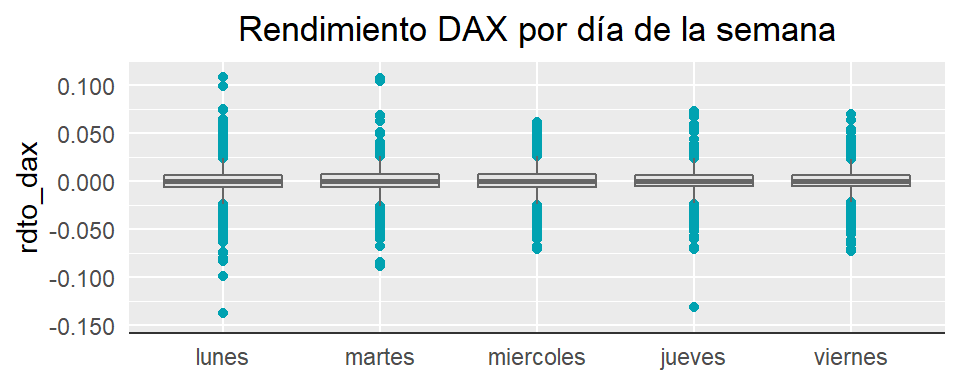
\includegraphics[width=0.9\linewidth]{RmdFigs/boxplot-dax-1} \end{center}

Se generan valores binarios para los días de la semana.

\begin{Shaded}
\begin{Highlighting}[]
\NormalTok{df_dax_nasdaq_dow_dummies <-}\StringTok{ }\NormalTok{df_dax_nasdaq_dow }\OperatorTok\StringTok{ }
\StringTok{  }\KeywordTok{mutate}\NormalTok{(}\DataTypeTok{var =} \DecValTok{1}\NormalTok{) }\OperatorTok\StringTok{                                   }\CommentTok{# Asigno un 1 en todas las filas de una columna}
\StringTok{  }\KeywordTok{spread}\NormalTok{(}\DataTypeTok{key =}\NormalTok{ dia, }\DataTypeTok{value =}\NormalTok{ var, }\DataTypeTok{fill =} \DecValTok{0}\NormalTok{) }\OperatorTok\StringTok{          }\CommentTok{# Creo las variables dummy }

\CommentTok{# Reordeno y elimino lunes}
\NormalTok{dplyr}\OperatorTok{::}\KeywordTok{select}\NormalTok{(Fecha, DAX, rdto_dax, NASDAQ, rdto_nasdaq, martes, miercoles, jueves, viernes)  }
\KeywordTok{head}\NormalTok{(df_dax_nasdaq_dow_dummies)}
\end{Highlighting}
\end{Shaded}

\begin{verbatim}
## # A tibble: 6 x 9
##   Fecha                 DAX rdto_dax NASDAQ rdto_nasdaq martes miercoles jueves
##   <dttm>              <dbl>    <dbl>  <dbl>       <dbl>  <dbl>     <dbl>  <dbl>
## 1 1971-02-05 00:00:00  508.  0         100     0             0         0      0
## 2 1971-02-08 00:00:00  510.  0.00242   101.    0.00836       0         0      0
## 3 1971-02-09 00:00:00  506. -0.00659   101.   -0.000794      1         0      0
## 4 1971-02-10 00:00:00  502. -0.00863   101.   -0.000695      0         1      0
## 5 1971-02-11 00:00:00  504.  0.00386   101.    0.00752       0         0      1
## 6 1971-02-12 00:00:00  513.  0.0180    102.    0.00590       0         0      0
## # ... with 1 more variable: viernes <dbl>
\end{verbatim}

\hypertarget{regresiuxf3n-muxednimo-cuadruxe1tica}{%
\section{Regresión mínimo
cuadrática}\label{regresiuxf3n-muxednimo-cuadruxe1tica}}

Para el cálculo de la regresión se descartan las columnas Fecha, DAX y
NASDAQ, quedando seleccionadas solamente las columnas de los días y la
correspondiente al Rendimiento DAX.

\begin{Shaded}
\begin{Highlighting}[]
\NormalTok{analysis_dax <-}\StringTok{ }\NormalTok{df_dax_nasdaq_dow_dummies }\OperatorTok\StringTok{ }\NormalTok{dplyr}\OperatorTok{::}\KeywordTok{select}\NormalTok{(}\OperatorTok{-}\NormalTok{Fecha,}\OperatorTok{-}\NormalTok{DAX,}\OperatorTok{-}\NormalTok{NASDAQ,}\OperatorTok{-}\NormalTok{rdto_nasdaq)}
\KeywordTok{head}\NormalTok{(analysis_dax)}
\end{Highlighting}
\end{Shaded}

\begin{verbatim}
## # A tibble: 6 x 5
##   rdto_dax martes miercoles jueves viernes
##      <dbl>  <dbl>     <dbl>  <dbl>   <dbl>
## 1  0            0         0      0       1
## 2  0.00242      0         0      0       0
## 3 -0.00659      1         0      0       0
## 4 -0.00863      0         1      0       0
## 5  0.00386      0         0      1       0
## 6  0.0180       0         0      0       1
\end{verbatim}

Se calculan los valores de correlación entre los días de la semana y el
rendimiento.

\begin{Shaded}
\begin{Highlighting}[]
\KeywordTok{cor}\NormalTok{(analysis_dax)}
\end{Highlighting}
\end{Shaded}

\begin{verbatim}
##               rdto_dax       martes    miercoles       jueves    viernes
## rdto_dax   1.000000000  0.006515476  0.006913422 -0.003329002  0.0115477
## martes     0.006515476  1.000000000 -0.250000000 -0.250000000 -0.2500000
## miercoles  0.006913422 -0.250000000  1.000000000 -0.250000000 -0.2500000
## jueves    -0.003329002 -0.250000000 -0.250000000  1.000000000 -0.2500000
## viernes    0.011547696 -0.250000000 -0.250000000 -0.250000000  1.0000000
\end{verbatim}

Se observa una correlación negativa del día jueves.

\begin{Shaded}
\begin{Highlighting}[]
\KeywordTok{library}\NormalTok{(GGally)}
\KeywordTok{ggpairs}\NormalTok{(analysis_dax, }\DataTypeTok{lower =} \KeywordTok{list}\NormalTok{(}\DataTypeTok{continuous =} \StringTok{"smooth"}\NormalTok{),}
        \DataTypeTok{diag =} \KeywordTok{list}\NormalTok{(}\DataTypeTok{continuous =} \StringTok{"barDiag"}\NormalTok{), }\DataTypeTok{axisLabels =} \StringTok{"none"}\NormalTok{)}
\end{Highlighting}
\end{Shaded}

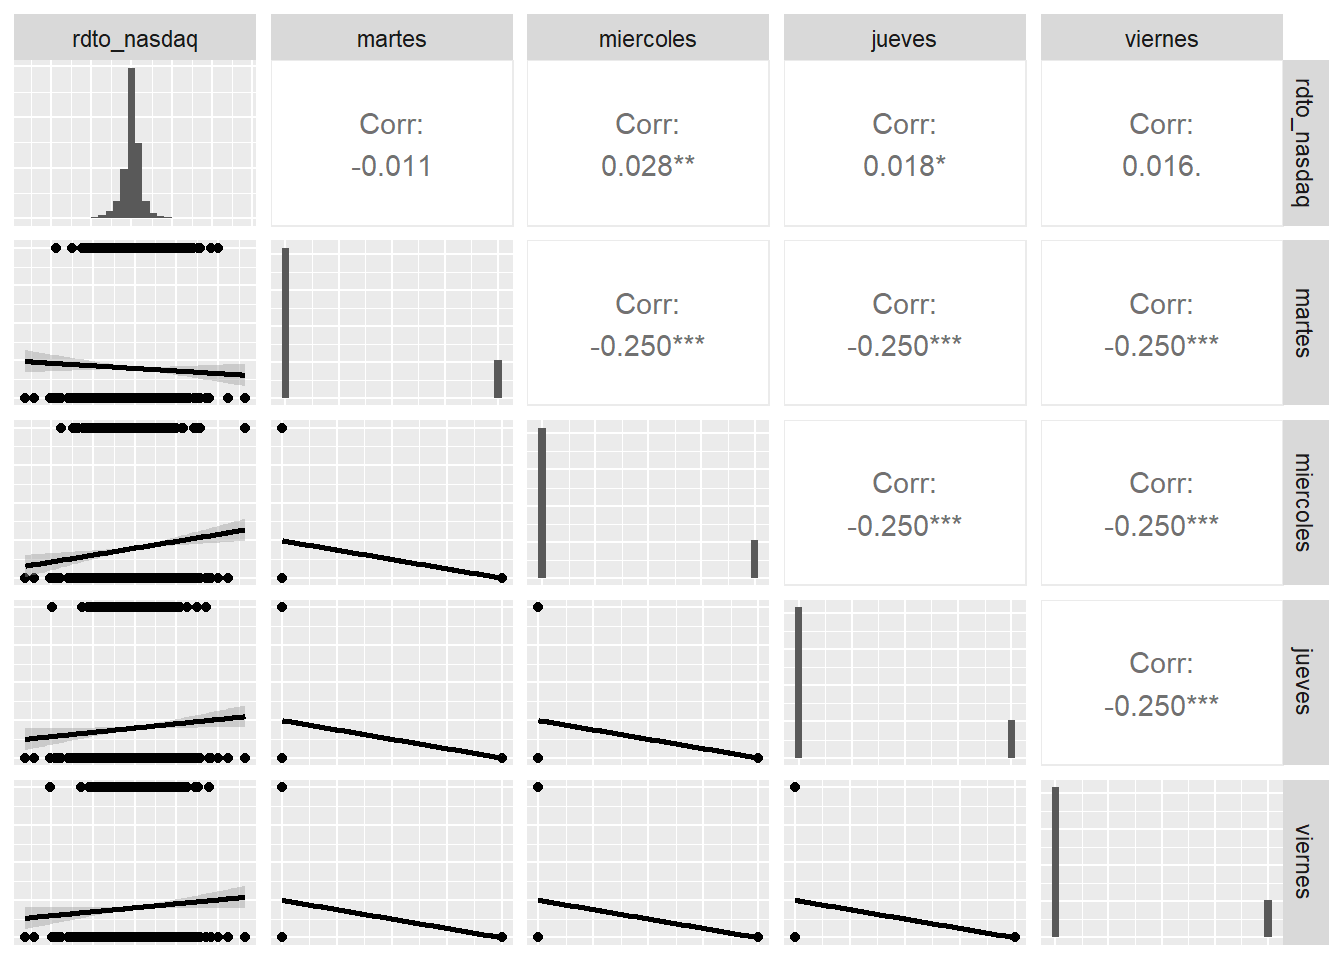
\includegraphics[width=0.9\linewidth]{RmdFigs/unnamed-chunk-5-1}

Se genera la regresión lineal con el objetivo de explicar los valores de
rdto\_dax en base a las variables dicotómicas independientes
correspondientes a los días de la semana. En este caso se tiene la
ecuación
\(R_t = \beta_2 M_t + \beta_3 X_t + \beta_4 J_t + \beta_5 V_t + \epsilon_t\)
Las variables \(M_t\), \(X_t\), \(J_t\) y \(V_t\) son las variables
dummy asociadas a los días de la semana, tomando valor 1 si la
observación corresponde a dicho día y 0 en otro caso. Los coeficientes
\(\beta_2, \beta_3, \beta_4\) y \(\beta_5\) representan los rendimientos
medios de cada día. El término de error se representa mediante
\(\epsilon_t\). En este caso se han considerado 4 variables dummys
correspondientes a los días martes, miércoles, jueves y viernes para
tratar de explicar la variabilidad de los rendimientos tomando como base
el día lunes.

Se configura y ejecuta el modelo.

\begin{Shaded}
\begin{Highlighting}[]
\NormalTok{full_model_dax <-}\StringTok{ }\KeywordTok{lm}\NormalTok{(rdto_dax }\OperatorTok{~}\StringTok{ }\NormalTok{martes }\OperatorTok{+}\StringTok{ }\NormalTok{miercoles }\OperatorTok{+}\StringTok{ }\NormalTok{jueves }\OperatorTok{+}\StringTok{ }\NormalTok{viernes, }\DataTypeTok{data =}\NormalTok{ analysis_dax)}
\KeywordTok{summary}\NormalTok{(full_model_dax)}
\end{Highlighting}
\end{Shaded}

\begin{verbatim}
## 
## Call:
## lm(formula = rdto_dax ~ martes + miercoles + jueves + viernes, 
##     data = analysis_dax)
## 
## Residuals:
##       Min        1Q    Median        3Q       Max 
## -0.136805 -0.005838  0.000177  0.006320  0.108268 
## 
## Coefficients:
##               Estimate Std. Error t value Pr(>|t|)  
## (Intercept) -0.0002937  0.0002466  -1.191   0.2337  
## martes       0.0007084  0.0003488   2.031   0.0423 *
## miercoles    0.0007185  0.0003488   2.060   0.0394 *
## jueves       0.0004608  0.0003488   1.321   0.1865  
## viernes      0.0008350  0.0003488   2.394   0.0167 *
## ---
## Signif. codes:  0 '***' 0.001 '**' 0.01 '*' 0.05 '.' 0.1 ' ' 1
## 
## Residual standard error: 0.01258 on 12995 degrees of freedom
## Multiple R-squared:  0.0005626,  Adjusted R-squared:  0.000255 
## F-statistic: 1.829 on 4 and 12995 DF,  p-value: 0.1202
\end{verbatim}

\#El modelo con las 4 variables dummys introducidas como predictores
tiene un valor de \(R_2\) bajo (0.00056). \#El p-value del estadístico F
no es significativo (0.1202). En los resultados se observa que el
p-value de la prueba de hipótesis del estadístico t para el día jueves
es 0.1865 (mayor que 0.05), lo que estaría indicando que la variabilidad
de los rendimientos no está relacionada con la variabilidad de los
jueves, al menos para estos datos.

Si se aplica la estrategia de stepwise mixto para selección de los
mejores predictores, se obtiene que el mejor modelo es lm(formula =
rdto\_dax \textasciitilde{} martes + miercoles + viernes, data =
analysis\_dax), lo que refuerza la evidencia de que el día jueves no
presenta valor explicativo.

\begin{Shaded}
\begin{Highlighting}[]
\KeywordTok{step}\NormalTok{(}\DataTypeTok{object =}\NormalTok{ full_model_dax, }\DataTypeTok{direction =} \StringTok{"both"}\NormalTok{, }\DataTypeTok{trace =} \DecValTok{1}\NormalTok{)}
\end{Highlighting}
\end{Shaded}

\begin{verbatim}
## Start:  AIC=-113769.2
## rdto_dax ~ martes + miercoles + jueves + viernes
## 
##             Df  Sum of Sq    RSS     AIC
## - jueves     1 0.00027604 2.0556 -113769
## <none>                    2.0554 -113769
## - martes     1 0.00065246 2.0560 -113767
## - miercoles  1 0.00067103 2.0560 -113767
## - viernes    1 0.00090646 2.0563 -113765
## 
## Step:  AIC=-113769.5
## rdto_dax ~ martes + miercoles + viernes
## 
##             Df  Sum of Sq    RSS     AIC
## <none>                    2.0556 -113769
## + jueves     1 0.00027604 2.0554 -113769
## - martes     1 0.00039611 2.0560 -113769
## - miercoles  1 0.00041287 2.0561 -113769
## - viernes    1 0.00063366 2.0563 -113767
\end{verbatim}

\begin{verbatim}
## 
## Call:
## lm(formula = rdto_dax ~ martes + miercoles + viernes, data = analysis_dax)
## 
## Coefficients:
## (Intercept)       martes    miercoles      viernes  
##  -6.332e-05    4.780e-04    4.881e-04    6.046e-04
\end{verbatim}

Se ejecuta la regresión lineal considerando las variables dummys se los
días martes, miércoles y viernes.

\begin{Shaded}
\begin{Highlighting}[]
\NormalTok{full_model_dax2 <-}\StringTok{ }\KeywordTok{lm}\NormalTok{(}\DataTypeTok{formula =}\NormalTok{ rdto_dax }\OperatorTok{~}\StringTok{ }\NormalTok{martes }\OperatorTok{+}\StringTok{ }\NormalTok{miercoles }\OperatorTok{+}\StringTok{ }\NormalTok{viernes, }\DataTypeTok{data =}\NormalTok{ analysis_dax)}
\KeywordTok{summary}\NormalTok{(full_model_dax2)}
\end{Highlighting}
\end{Shaded}

\begin{verbatim}
## 
## Call:
## lm(formula = rdto_dax ~ martes + miercoles + viernes, data = analysis_dax)
## 
## Residuals:
##       Min        1Q    Median        3Q       Max 
## -0.137036 -0.005814  0.000063  0.006311  0.108038 
## 
## Coefficients:
##               Estimate Std. Error t value Pr(>|t|)  
## (Intercept) -6.332e-05  1.744e-04  -0.363   0.7166  
## martes       4.780e-04  3.021e-04   1.582   0.1136  
## miercoles    4.881e-04  3.021e-04   1.616   0.1062  
## viernes      6.046e-04  3.021e-04   2.002   0.0454 *
## ---
## Signif. codes:  0 '***' 0.001 '**' 0.01 '*' 0.05 '.' 0.1 ' ' 1
## 
## Residual standard error: 0.01258 on 12996 degrees of freedom
## Multiple R-squared:  0.0004284,  Adjusted R-squared:  0.0001977 
## F-statistic: 1.857 on 3 and 12996 DF,  p-value: 0.1346
\end{verbatim}

Al aplicar este modelo se obtiene el p-value de la prueba de hipótesis
del estadístico t para el día viernes = 0.0454 (menor que 0.05), lo que
estaría indicando, con un nivel de significancia de 0.05 que hay un
efecto del día viernes.

\hypertarget{regresiuxf3n-incorporando-la-ecuaciuxf3n-de-varianza-como-un-modelo-garch11}{%
\section{REGRESIÓN INCORPORANDO LA ECUACIÓN DE VARIANZA COMO UN MODELO
GARCH(1,1)}\label{regresiuxf3n-incorporando-la-ecuaciuxf3n-de-varianza-como-un-modelo-garch11}}

Se generan los vectores de rendimiento para DAX y los vectores de los
días martes a viernes.

\begin{Shaded}
\begin{Highlighting}[]
\NormalTok{n <-}\StringTok{ }\KeywordTok{nrow}\NormalTok{(df_dax_nasdaq_dow_dummies)}

\NormalTok{rdto_dax <-}\StringTok{ }\KeywordTok{as.numeric}\NormalTok{(}\KeywordTok{unlist}\NormalTok{(df_dax_nasdaq_dow_dummies[}\DecValTok{2}\OperatorTok{:}\NormalTok{n,}\StringTok{"rdto_dax"}\NormalTok{]))}

\NormalTok{vardias_ma <-}\StringTok{ }\KeywordTok{as.numeric}\NormalTok{(}\KeywordTok{unlist}\NormalTok{(df_dax_nasdaq_dow_dummies[}\DecValTok{2}\OperatorTok{:}\NormalTok{n,}\StringTok{"martes"}\NormalTok{]))}
\NormalTok{vardias_mi <-}\StringTok{ }\KeywordTok{as.numeric}\NormalTok{(}\KeywordTok{unlist}\NormalTok{(df_dax_nasdaq_dow_dummies[}\DecValTok{2}\OperatorTok{:}\NormalTok{n,}\StringTok{"miercoles"}\NormalTok{]))}
\NormalTok{vardias_ju <-}\StringTok{ }\KeywordTok{as.numeric}\NormalTok{(}\KeywordTok{unlist}\NormalTok{(df_dax_nasdaq_dow_dummies[}\DecValTok{2}\OperatorTok{:}\NormalTok{n,}\StringTok{"jueves"}\NormalTok{]))}
\NormalTok{vardias_vi <-}\StringTok{ }\KeywordTok{as.numeric}\NormalTok{(}\KeywordTok{unlist}\NormalTok{(df_dax_nasdaq_dow_dummies[}\DecValTok{2}\OperatorTok{:}\NormalTok{n,}\StringTok{"viernes"}\NormalTok{]))}

\NormalTok{vardias <-}\StringTok{ }\KeywordTok{cbind}\NormalTok{(vardias_ma,vardias_mi,vardias_ju,vardias_vi)}
\end{Highlighting}
\end{Shaded}

Se prueban distintos modelos para analizarlos, se analizan si los
residuos son ruido blanco y se seleccionan los modelos mas adecuados.

\hypertarget{modelo-sgarch11-con-external-regressors-en-modelo-de-media.-distribuciuxf3n-std.}{%
\subsection{Modelo sGARCH(1,1) con External Regressors en modelo de
media. Distribución
std.}\label{modelo-sgarch11-con-external-regressors-en-modelo-de-media.-distribuciuxf3n-std.}}

\begin{Shaded}
\begin{Highlighting}[]
\NormalTok{spec_dax1 <-}\StringTok{ }\KeywordTok{ugarchspec}\NormalTok{(}\DataTypeTok{variance.model =} \KeywordTok{list}\NormalTok{(}\DataTypeTok{model =} \StringTok{"sGARCH"}\NormalTok{, }\DataTypeTok{garchOrder =} \KeywordTok{c}\NormalTok{(}\DecValTok{1}\NormalTok{, }\DecValTok{1}\NormalTok{), }
                        \DataTypeTok{submodel =} \OtherTok{NULL}\NormalTok{, }\DataTypeTok{external.regressors =} \OtherTok{NULL}\NormalTok{, }\DataTypeTok{variance.targeting =} \OtherTok{FALSE}\NormalTok{), }
                        \DataTypeTok{mean.model =} \KeywordTok{list}\NormalTok{(}\DataTypeTok{armaOrder =} \KeywordTok{c}\NormalTok{(}\DecValTok{0}\NormalTok{, }\DecValTok{0}\NormalTok{),}\DataTypeTok{external.regressors =}\NormalTok{ vardias[,}\DecValTok{1}\OperatorTok{:}\DecValTok{4}\NormalTok{]),}
                        \DataTypeTok{distribution.model =} \StringTok{"std"}\NormalTok{)}
\NormalTok{garch_dax1 <-}\StringTok{ }\KeywordTok{ugarchfit}\NormalTok{(}\DataTypeTok{spec=}\NormalTok{spec_dax1,}\DataTypeTok{data=}\NormalTok{rdto_dax)}
\end{Highlighting}
\end{Shaded}

\hypertarget{modelo-sgarch11-con-external-regressors-en-modelo-de-media-y-de-varianza.-distribuciuxf3n-std}{%
\subsection{Modelo sGARCH(1,1) con External Regressors en modelo de
media y de varianza. Distribución
std}\label{modelo-sgarch11-con-external-regressors-en-modelo-de-media-y-de-varianza.-distribuciuxf3n-std}}

\begin{Shaded}
\begin{Highlighting}[]
\NormalTok{spec_dax1_2er <-}\StringTok{ }\KeywordTok{ugarchspec}\NormalTok{(}\DataTypeTok{variance.model =} \KeywordTok{list}\NormalTok{(}\DataTypeTok{model =} \StringTok{"sGARCH"}\NormalTok{, }\DataTypeTok{garchOrder =} \KeywordTok{c}\NormalTok{(}\DecValTok{1}\NormalTok{, }\DecValTok{1}\NormalTok{), }
                        \DataTypeTok{submodel =} \OtherTok{NULL}\NormalTok{, }\DataTypeTok{external.regressors =}\NormalTok{ vardias[,}\DecValTok{1}\OperatorTok{:}\DecValTok{4}\NormalTok{], }\DataTypeTok{variance.targeting =} \OtherTok{FALSE}\NormalTok{), }
                        \DataTypeTok{mean.model =} \KeywordTok{list}\NormalTok{(}\DataTypeTok{armaOrder =} \KeywordTok{c}\NormalTok{(}\DecValTok{0}\NormalTok{, }\DecValTok{0}\NormalTok{),}\DataTypeTok{external.regressors =}\NormalTok{ vardias[,}\DecValTok{1}\OperatorTok{:}\DecValTok{4}\NormalTok{]),}
                        \DataTypeTok{distribution.model =} \StringTok{"std"}\NormalTok{)}
\NormalTok{garch_dax1_2er <-}\StringTok{ }\KeywordTok{ugarchfit}\NormalTok{(}\DataTypeTok{spec=}\NormalTok{spec_dax1_2er,}\DataTypeTok{data=}\NormalTok{rdto_dax)}
\end{Highlighting}
\end{Shaded}

\hypertarget{modelo-gjrgarch11-con-external-regressors-en-modelo-de-media.-distribuciuxf3n-std}{%
\subsection{Modelo gjrGARCH(1,1) con External Regressors en modelo de
media. Distribución
std}\label{modelo-gjrgarch11-con-external-regressors-en-modelo-de-media.-distribuciuxf3n-std}}

\begin{Shaded}
\begin{Highlighting}[]
\NormalTok{spec_dax2 <-}\StringTok{ }\KeywordTok{ugarchspec}\NormalTok{(}\DataTypeTok{variance.model =} \KeywordTok{list}\NormalTok{(}\DataTypeTok{model =} \StringTok{"gjrGARCH"}\NormalTok{, }\DataTypeTok{garchOrder =} \KeywordTok{c}\NormalTok{(}\DecValTok{1}\NormalTok{, }\DecValTok{1}\NormalTok{), }
                    \DataTypeTok{submodel =} \OtherTok{NULL}\NormalTok{, }\DataTypeTok{external.regressors =} \OtherTok{NULL}\NormalTok{, }\DataTypeTok{variance.targeting =} \OtherTok{FALSE}\NormalTok{), }
                    \DataTypeTok{mean.model =} \KeywordTok{list}\NormalTok{(}\DataTypeTok{armaOrder =} \KeywordTok{c}\NormalTok{(}\DecValTok{0}\NormalTok{, }\DecValTok{0}\NormalTok{),}\DataTypeTok{external.regressors =}\NormalTok{ vardias[,}\DecValTok{1}\OperatorTok{:}\DecValTok{4}\NormalTok{]),}
               \DataTypeTok{distribution.model =} \StringTok{"std"}\NormalTok{)}
\NormalTok{garch_dax2 <-}\StringTok{ }\KeywordTok{ugarchfit}\NormalTok{(}\DataTypeTok{spec=}\NormalTok{spec_dax2,}\DataTypeTok{data=}\NormalTok{rdto_dax)}
\end{Highlighting}
\end{Shaded}

\hypertarget{modelo-gjrgarch11-con-external-regressors-en-modelo-de-media-y-de-varianza.-distribuciuxf3n-std}{%
\subsection{Modelo gjrGARCH(1,1) con External Regressors en modelo de
media y de varianza. Distribución
std}\label{modelo-gjrgarch11-con-external-regressors-en-modelo-de-media-y-de-varianza.-distribuciuxf3n-std}}

\begin{Shaded}
\begin{Highlighting}[]
\NormalTok{spec_dax2_2er <-}\StringTok{ }\KeywordTok{ugarchspec}\NormalTok{(}\DataTypeTok{variance.model =} \KeywordTok{list}\NormalTok{(}\DataTypeTok{model =} \StringTok{"gjrGARCH"}\NormalTok{, }\DataTypeTok{garchOrder =} \KeywordTok{c}\NormalTok{(}\DecValTok{1}\NormalTok{, }\DecValTok{1}\NormalTok{), }
                    \DataTypeTok{submodel =} \OtherTok{NULL}\NormalTok{, }\DataTypeTok{external.regressors  =}\NormalTok{ vardias[,}\DecValTok{1}\OperatorTok{:}\DecValTok{4}\NormalTok{], }\DataTypeTok{variance.targeting =} \OtherTok{FALSE}\NormalTok{), }
                    \DataTypeTok{mean.model =} \KeywordTok{list}\NormalTok{(}\DataTypeTok{armaOrder =} \KeywordTok{c}\NormalTok{(}\DecValTok{0}\NormalTok{, }\DecValTok{0}\NormalTok{),}\DataTypeTok{external.regressors =}\NormalTok{ vardias[,}\DecValTok{1}\OperatorTok{:}\DecValTok{4}\NormalTok{]),}
               \DataTypeTok{distribution.model =} \StringTok{"std"}\NormalTok{)}
\NormalTok{garch_dax2_2er <-}\StringTok{ }\KeywordTok{ugarchfit}\NormalTok{(}\DataTypeTok{spec=}\NormalTok{spec_dax2_2er,}\DataTypeTok{data=}\NormalTok{rdto_dax)}
\end{Highlighting}
\end{Shaded}

\hypertarget{modelo-egarch11-con-external-regressors-en-modelo-de-media.-distribuciuxf3n-std}{%
\subsection{Modelo eGARCH(1,1) con External Regressors en modelo de
media. Distribución
std}\label{modelo-egarch11-con-external-regressors-en-modelo-de-media.-distribuciuxf3n-std}}

\begin{Shaded}
\begin{Highlighting}[]
\NormalTok{spec_dax3 <-}\StringTok{ }\KeywordTok{ugarchspec}\NormalTok{(}\DataTypeTok{variance.model =} \KeywordTok{list}\NormalTok{(}\DataTypeTok{model =} \StringTok{"eGARCH"}\NormalTok{, }\DataTypeTok{garchOrder =} \KeywordTok{c}\NormalTok{(}\DecValTok{1}\NormalTok{, }\DecValTok{1}\NormalTok{), }
                    \DataTypeTok{submodel =} \OtherTok{NULL}\NormalTok{, }\DataTypeTok{external.regressors =} \OtherTok{NULL}\NormalTok{, }\DataTypeTok{variance.targeting =} \OtherTok{FALSE}\NormalTok{), }
                    \DataTypeTok{mean.model =} \KeywordTok{list}\NormalTok{(}\DataTypeTok{armaOrder =} \KeywordTok{c}\NormalTok{(}\DecValTok{0}\NormalTok{, }\DecValTok{0}\NormalTok{),}\DataTypeTok{external.regressors =}\NormalTok{ vardias[,}\DecValTok{1}\OperatorTok{:}\DecValTok{4}\NormalTok{]),}
               \DataTypeTok{distribution.model =} \StringTok{"std"}\NormalTok{)}
\NormalTok{garch_dax3 <-}\StringTok{ }\KeywordTok{ugarchfit}\NormalTok{(}\DataTypeTok{spec=}\NormalTok{spec_dax3,}\DataTypeTok{data=}\NormalTok{rdto_dax)}
\end{Highlighting}
\end{Shaded}

\hypertarget{modelo-egarch11-con-external-regressors-en-modelo-de-media-y-de-varianza.-distribuciuxf3n-std}{%
\subsection{Modelo eGARCH(1,1) con External Regressors en modelo de
media y de varianza. Distribución
std}\label{modelo-egarch11-con-external-regressors-en-modelo-de-media-y-de-varianza.-distribuciuxf3n-std}}

\begin{Shaded}
\begin{Highlighting}[]
\NormalTok{spec_dax3_2er <-}\StringTok{ }\KeywordTok{ugarchspec}\NormalTok{(}\DataTypeTok{variance.model =} \KeywordTok{list}\NormalTok{(}\DataTypeTok{model =} \StringTok{"eGARCH"}\NormalTok{, }\DataTypeTok{garchOrder =} \KeywordTok{c}\NormalTok{(}\DecValTok{1}\NormalTok{, }\DecValTok{1}\NormalTok{), }
                    \DataTypeTok{submodel =} \OtherTok{NULL}\NormalTok{, }\DataTypeTok{external.regressors =}\NormalTok{ vardias[,}\DecValTok{1}\OperatorTok{:}\DecValTok{4}\NormalTok{], }\DataTypeTok{variance.targeting =} \OtherTok{FALSE}\NormalTok{), }
                    \DataTypeTok{mean.model =} \KeywordTok{list}\NormalTok{(}\DataTypeTok{armaOrder =} \KeywordTok{c}\NormalTok{(}\DecValTok{0}\NormalTok{, }\DecValTok{0}\NormalTok{),}\DataTypeTok{external.regressors =}\NormalTok{ vardias[,}\DecValTok{1}\OperatorTok{:}\DecValTok{4}\NormalTok{]),}
               \DataTypeTok{distribution.model =} \StringTok{"std"}\NormalTok{)}
\NormalTok{garch_dax3_2er <-}\StringTok{ }\KeywordTok{ugarchfit}\NormalTok{(}\DataTypeTok{spec=}\NormalTok{spec_dax3_2er,}\DataTypeTok{data=}\NormalTok{rdto_dax)}
\end{Highlighting}
\end{Shaded}

\hypertarget{modelo-sgarch11-con-external-regressors-en-modelo-de-media.-distribuciuxf3n-norm}{%
\subsection{Modelo sGARCH(1,1) con External Regressors en modelo de
media. Distribución
norm}\label{modelo-sgarch11-con-external-regressors-en-modelo-de-media.-distribuciuxf3n-norm}}

\begin{Shaded}
\begin{Highlighting}[]
\NormalTok{spec_dax4 <-}\StringTok{ }\KeywordTok{ugarchspec}\NormalTok{(}\DataTypeTok{variance.model =} \KeywordTok{list}\NormalTok{(}\DataTypeTok{model =} \StringTok{"sGARCH"}\NormalTok{, }\DataTypeTok{garchOrder =} \KeywordTok{c}\NormalTok{(}\DecValTok{1}\NormalTok{, }\DecValTok{1}\NormalTok{), }
                    \DataTypeTok{submodel =} \OtherTok{NULL}\NormalTok{, }\DataTypeTok{external.regressors =} \OtherTok{NULL}\NormalTok{, }\DataTypeTok{variance.targeting =} \OtherTok{FALSE}\NormalTok{), }
                    \DataTypeTok{mean.model =} \KeywordTok{list}\NormalTok{(}\DataTypeTok{armaOrder =} \KeywordTok{c}\NormalTok{(}\DecValTok{0}\NormalTok{, }\DecValTok{0}\NormalTok{),}\DataTypeTok{external.regressors =}\NormalTok{ vardias[,}\DecValTok{1}\OperatorTok{:}\DecValTok{4}\NormalTok{]),}
               \DataTypeTok{distribution.model =} \StringTok{"norm"}\NormalTok{)}
\NormalTok{garch_dax4 <-}\StringTok{ }\KeywordTok{ugarchfit}\NormalTok{(}\DataTypeTok{spec=}\NormalTok{spec_dax4,}\DataTypeTok{data=}\NormalTok{rdto_dax)}
\end{Highlighting}
\end{Shaded}

\hypertarget{modelo-sgarch11-con-external-regressors-en-modelo-de-media-y-de-varianza.-distribuciuxf3n-norm}{%
\subsection{Modelo sGARCH(1,1) con External Regressors en modelo de
media y de varianza. Distribución
norm}\label{modelo-sgarch11-con-external-regressors-en-modelo-de-media-y-de-varianza.-distribuciuxf3n-norm}}

\begin{Shaded}
\begin{Highlighting}[]
\NormalTok{spec_dax4_2er <-}\StringTok{ }\KeywordTok{ugarchspec}\NormalTok{(}\DataTypeTok{variance.model =} \KeywordTok{list}\NormalTok{(}\DataTypeTok{model =} \StringTok{"sGARCH"}\NormalTok{, }\DataTypeTok{garchOrder =} \KeywordTok{c}\NormalTok{(}\DecValTok{1}\NormalTok{, }\DecValTok{1}\NormalTok{), }
                    \DataTypeTok{submodel =} \OtherTok{NULL}\NormalTok{, }\DataTypeTok{external.regressors =}\NormalTok{ vardias[,}\DecValTok{1}\OperatorTok{:}\DecValTok{4}\NormalTok{], }\DataTypeTok{variance.targeting =} \OtherTok{FALSE}\NormalTok{), }
                    \DataTypeTok{mean.model =} \KeywordTok{list}\NormalTok{(}\DataTypeTok{armaOrder =} \KeywordTok{c}\NormalTok{(}\DecValTok{0}\NormalTok{, }\DecValTok{0}\NormalTok{),}\DataTypeTok{external.regressors =}\NormalTok{ vardias[,}\DecValTok{1}\OperatorTok{:}\DecValTok{4}\NormalTok{]),}
               \DataTypeTok{distribution.model =} \StringTok{"norm"}\NormalTok{)}
\NormalTok{garch_dax4_2er <-}\StringTok{ }\KeywordTok{ugarchfit}\NormalTok{(}\DataTypeTok{spec=}\NormalTok{spec_dax4_2er,}\DataTypeTok{data=}\NormalTok{rdto_dax)}
\end{Highlighting}
\end{Shaded}

\hypertarget{modelo-gjrgarch11-con-external-regressors-en-modelo-de-media.-distribuciuxf3n-norm}{%
\subsection{Modelo gjrGARCH(1,1) con External Regressors en modelo de
media. Distribución
norm}\label{modelo-gjrgarch11-con-external-regressors-en-modelo-de-media.-distribuciuxf3n-norm}}

\begin{Shaded}
\begin{Highlighting}[]
\NormalTok{spec_dax5 <-}\StringTok{ }\KeywordTok{ugarchspec}\NormalTok{(}\DataTypeTok{variance.model =} \KeywordTok{list}\NormalTok{(}\DataTypeTok{model =} \StringTok{"gjrGARCH"}\NormalTok{, }\DataTypeTok{garchOrder =} \KeywordTok{c}\NormalTok{(}\DecValTok{1}\NormalTok{, }\DecValTok{1}\NormalTok{), }
                    \DataTypeTok{submodel =} \OtherTok{NULL}\NormalTok{, }\DataTypeTok{external.regressors =} \OtherTok{NULL}\NormalTok{, }\DataTypeTok{variance.targeting =} \OtherTok{FALSE}\NormalTok{), }
                    \DataTypeTok{mean.model =} \KeywordTok{list}\NormalTok{(}\DataTypeTok{armaOrder =} \KeywordTok{c}\NormalTok{(}\DecValTok{0}\NormalTok{, }\DecValTok{0}\NormalTok{),}\DataTypeTok{external.regressors =}\NormalTok{ vardias[,}\DecValTok{1}\OperatorTok{:}\DecValTok{4}\NormalTok{]),}
               \DataTypeTok{distribution.model =} \StringTok{"norm"}\NormalTok{)}
\NormalTok{garch_dax5 <-}\StringTok{ }\KeywordTok{ugarchfit}\NormalTok{(}\DataTypeTok{spec=}\NormalTok{spec_dax5,}\DataTypeTok{data=}\NormalTok{rdto_dax)}
\end{Highlighting}
\end{Shaded}

\hypertarget{modelo-gjrgarch11-con-external-regressors-en-modelo-de-media-y-de-varianza.-distribuciuxf3n-norm}{%
\subsection{Modelo gjrGARCH(1,1) con External Regressors en modelo de
media y de varianza. Distribución
norm}\label{modelo-gjrgarch11-con-external-regressors-en-modelo-de-media-y-de-varianza.-distribuciuxf3n-norm}}

\begin{Shaded}
\begin{Highlighting}[]
\NormalTok{spec_dax5_2er <-}\StringTok{ }\KeywordTok{ugarchspec}\NormalTok{(}\DataTypeTok{variance.model =} \KeywordTok{list}\NormalTok{(}\DataTypeTok{model =} \StringTok{"gjrGARCH"}\NormalTok{, }\DataTypeTok{garchOrder =} \KeywordTok{c}\NormalTok{(}\DecValTok{1}\NormalTok{, }\DecValTok{1}\NormalTok{), }
                    \DataTypeTok{submodel =} \OtherTok{NULL}\NormalTok{, }\DataTypeTok{external.regressors =}\NormalTok{ vardias[,}\DecValTok{1}\OperatorTok{:}\DecValTok{4}\NormalTok{], }\DataTypeTok{variance.targeting =} \OtherTok{FALSE}\NormalTok{), }
                    \DataTypeTok{mean.model =} \KeywordTok{list}\NormalTok{(}\DataTypeTok{armaOrder =} \KeywordTok{c}\NormalTok{(}\DecValTok{0}\NormalTok{, }\DecValTok{0}\NormalTok{),}\DataTypeTok{external.regressors =}\NormalTok{ vardias[,}\DecValTok{1}\OperatorTok{:}\DecValTok{4}\NormalTok{]),}
               \DataTypeTok{distribution.model =} \StringTok{"norm"}\NormalTok{)}
\NormalTok{garch_dax5_2er <-}\StringTok{ }\KeywordTok{ugarchfit}\NormalTok{(}\DataTypeTok{spec=}\NormalTok{spec_dax5_2er,}\DataTypeTok{data=}\NormalTok{rdto_dax)}
\end{Highlighting}
\end{Shaded}

\hypertarget{modelo-egarch11-con-external-regressors-en-modelo-de-media.-distribuciuxf3n-norm}{%
\subsection{Modelo eGARCH(1,1) con External Regressors en modelo de
media. Distribución
norm}\label{modelo-egarch11-con-external-regressors-en-modelo-de-media.-distribuciuxf3n-norm}}

\begin{Shaded}
\begin{Highlighting}[]
\NormalTok{spec_dax6 <-}\StringTok{ }\KeywordTok{ugarchspec}\NormalTok{(}\DataTypeTok{variance.model =} \KeywordTok{list}\NormalTok{(}\DataTypeTok{model =} \StringTok{"eGARCH"}\NormalTok{, }\DataTypeTok{garchOrder =} \KeywordTok{c}\NormalTok{(}\DecValTok{1}\NormalTok{, }\DecValTok{1}\NormalTok{), }
                    \DataTypeTok{submodel =} \OtherTok{NULL}\NormalTok{, }\DataTypeTok{external.regressors =} \OtherTok{NULL}\NormalTok{, }\DataTypeTok{variance.targeting =} \OtherTok{FALSE}\NormalTok{), }
                    \DataTypeTok{mean.model =} \KeywordTok{list}\NormalTok{(}\DataTypeTok{armaOrder =} \KeywordTok{c}\NormalTok{(}\DecValTok{0}\NormalTok{, }\DecValTok{0}\NormalTok{),}\DataTypeTok{external.regressors =}\NormalTok{ vardias[,}\DecValTok{1}\OperatorTok{:}\DecValTok{4}\NormalTok{]),}
               \DataTypeTok{distribution.model =} \StringTok{"norm"}\NormalTok{)}
\NormalTok{garch_dax6 <-}\StringTok{ }\KeywordTok{ugarchfit}\NormalTok{(}\DataTypeTok{spec=}\NormalTok{spec_dax6,}\DataTypeTok{data=}\NormalTok{rdto_dax)}
\end{Highlighting}
\end{Shaded}

\hypertarget{modelo-egarch11-con-external-regressors-en-modelo-de-media-y-de-varianza.-distribuciuxf3n-norm}{%
\subsection{Modelo eGARCH(1,1) con External Regressors en modelo de
media y de varianza. Distribución
norm}\label{modelo-egarch11-con-external-regressors-en-modelo-de-media-y-de-varianza.-distribuciuxf3n-norm}}

\begin{Shaded}
\begin{Highlighting}[]
\NormalTok{spec_dax6_2er <-}\StringTok{ }\KeywordTok{ugarchspec}\NormalTok{(}\DataTypeTok{variance.model =} \KeywordTok{list}\NormalTok{(}\DataTypeTok{model =} \StringTok{"eGARCH"}\NormalTok{, }\DataTypeTok{garchOrder =} \KeywordTok{c}\NormalTok{(}\DecValTok{1}\NormalTok{, }\DecValTok{1}\NormalTok{), }
                    \DataTypeTok{submodel =} \OtherTok{NULL}\NormalTok{, }\DataTypeTok{external.regressors =}\NormalTok{ vardias[,}\DecValTok{1}\OperatorTok{:}\DecValTok{4}\NormalTok{], }\DataTypeTok{variance.targeting =} \OtherTok{FALSE}\NormalTok{), }
                    \DataTypeTok{mean.model =} \KeywordTok{list}\NormalTok{(}\DataTypeTok{armaOrder =} \KeywordTok{c}\NormalTok{(}\DecValTok{0}\NormalTok{, }\DecValTok{0}\NormalTok{),}\DataTypeTok{external.regressors =}\NormalTok{ vardias[,}\DecValTok{1}\OperatorTok{:}\DecValTok{4}\NormalTok{]),}
               \DataTypeTok{distribution.model =} \StringTok{"norm"}\NormalTok{)}
\NormalTok{garch_dax6_2er <-}\StringTok{ }\KeywordTok{ugarchfit}\NormalTok{(}\DataTypeTok{spec=}\NormalTok{spec_dax6_2er,}\DataTypeTok{data=}\NormalTok{rdto_dax)}
\end{Highlighting}
\end{Shaded}

\hypertarget{modelos-garch11-con-arma10}{%
\section{Modelos GARCH(1,1) con
ARMA(1,0)}\label{modelos-garch11-con-arma10}}

\hypertarget{modelo-sgarch11-con-arma10-con-external-regressors-en-modelo-de-media.-distribuciuxf3n-std}{%
\subsection{Modelo sGARCH(1,1) con ARMA(1,0) con External Regressors en
modelo de media. Distribución
std}\label{modelo-sgarch11-con-arma10-con-external-regressors-en-modelo-de-media.-distribuciuxf3n-std}}

\begin{Shaded}
\begin{Highlighting}[]
\NormalTok{spec_dax1_ar1 <-}\StringTok{ }\KeywordTok{ugarchspec}\NormalTok{(}\DataTypeTok{variance.model =} \KeywordTok{list}\NormalTok{(}\DataTypeTok{model =} \StringTok{"sGARCH"}\NormalTok{, }\DataTypeTok{garchOrder =} \KeywordTok{c}\NormalTok{(}\DecValTok{1}\NormalTok{, }\DecValTok{1}\NormalTok{), }
                        \DataTypeTok{submodel =} \OtherTok{NULL}\NormalTok{, }\DataTypeTok{external.regressors =} \OtherTok{NULL}\NormalTok{, }\DataTypeTok{variance.targeting =} \OtherTok{FALSE}\NormalTok{), }
                        \DataTypeTok{mean.model =} \KeywordTok{list}\NormalTok{(}\DataTypeTok{armaOrder =} \KeywordTok{c}\NormalTok{(}\DecValTok{1}\NormalTok{, }\DecValTok{0}\NormalTok{),}\DataTypeTok{external.regressors =}\NormalTok{ vardias[,}\DecValTok{1}\OperatorTok{:}\DecValTok{4}\NormalTok{]),}
                        \DataTypeTok{distribution.model =} \StringTok{"std"}\NormalTok{)}
\NormalTok{garch_dax1_ar1 <-}\StringTok{ }\KeywordTok{ugarchfit}\NormalTok{(}\DataTypeTok{spec=}\NormalTok{spec_dax1_ar1,}\DataTypeTok{data=}\NormalTok{rdto_dax)}
\end{Highlighting}
\end{Shaded}

\hypertarget{modelo-sgarch11-con-arma10-con-external-regressors-en-modelo-de-media-y-de-varianza.-distribuciuxf3n-std}{%
\subsection{Modelo sGARCH(1,1) con ARMA(1,0) con External Regressors en
modelo de media y de varianza. Distribución
std}\label{modelo-sgarch11-con-arma10-con-external-regressors-en-modelo-de-media-y-de-varianza.-distribuciuxf3n-std}}

\begin{Shaded}
\begin{Highlighting}[]
\NormalTok{spec_dax1_2er_ar1 <-}\StringTok{ }\KeywordTok{ugarchspec}\NormalTok{(}\DataTypeTok{variance.model =} \KeywordTok{list}\NormalTok{(}\DataTypeTok{model =} \StringTok{"sGARCH"}\NormalTok{, }\DataTypeTok{garchOrder =} \KeywordTok{c}\NormalTok{(}\DecValTok{1}\NormalTok{, }\DecValTok{1}\NormalTok{), }
                        \DataTypeTok{submodel =} \OtherTok{NULL}\NormalTok{, }\DataTypeTok{external.regressors =}\NormalTok{ vardias[,}\DecValTok{1}\OperatorTok{:}\DecValTok{4}\NormalTok{], }\DataTypeTok{variance.targeting =} \OtherTok{FALSE}\NormalTok{), }
                        \DataTypeTok{mean.model =} \KeywordTok{list}\NormalTok{(}\DataTypeTok{armaOrder =} \KeywordTok{c}\NormalTok{(}\DecValTok{1}\NormalTok{, }\DecValTok{0}\NormalTok{),}\DataTypeTok{external.regressors =}\NormalTok{ vardias[,}\DecValTok{1}\OperatorTok{:}\DecValTok{4}\NormalTok{]),}
                        \DataTypeTok{distribution.model =} \StringTok{"std"}\NormalTok{)}
\NormalTok{garch_dax1_2er_ar1 <-}\StringTok{ }\KeywordTok{ugarchfit}\NormalTok{(}\DataTypeTok{spec=}\NormalTok{spec_dax1_2er_ar1,}\DataTypeTok{data=}\NormalTok{rdto_dax)}
\end{Highlighting}
\end{Shaded}

\hypertarget{modelo-gjrgarch11-con-arma10-con-external-regressors-en-modelo-de-media.-distribuciuxf3n-std}{%
\subsection{Modelo gjrGARCH(1,1) con ARMA(1,0) con External Regressors
en modelo de media. Distribución
std}\label{modelo-gjrgarch11-con-arma10-con-external-regressors-en-modelo-de-media.-distribuciuxf3n-std}}

\begin{Shaded}
\begin{Highlighting}[]
\NormalTok{spec_dax2_ar1 <-}\StringTok{ }\KeywordTok{ugarchspec}\NormalTok{(}\DataTypeTok{variance.model =} \KeywordTok{list}\NormalTok{(}\DataTypeTok{model =} \StringTok{"gjrGARCH"}\NormalTok{, }\DataTypeTok{garchOrder =} \KeywordTok{c}\NormalTok{(}\DecValTok{1}\NormalTok{, }\DecValTok{1}\NormalTok{), }
                    \DataTypeTok{submodel =} \OtherTok{NULL}\NormalTok{, }\DataTypeTok{external.regressors =} \OtherTok{NULL}\NormalTok{, }\DataTypeTok{variance.targeting =} \OtherTok{FALSE}\NormalTok{), }
                    \DataTypeTok{mean.model =} \KeywordTok{list}\NormalTok{(}\DataTypeTok{armaOrder =} \KeywordTok{c}\NormalTok{(}\DecValTok{1}\NormalTok{, }\DecValTok{0}\NormalTok{),}\DataTypeTok{external.regressors =}\NormalTok{ vardias[,}\DecValTok{1}\OperatorTok{:}\DecValTok{4}\NormalTok{]),}
               \DataTypeTok{distribution.model =} \StringTok{"std"}\NormalTok{)}
\NormalTok{garch_dax2_ar1 <-}\StringTok{ }\KeywordTok{ugarchfit}\NormalTok{(}\DataTypeTok{spec=}\NormalTok{spec_dax2_ar1,}\DataTypeTok{data=}\NormalTok{rdto_dax)}
\end{Highlighting}
\end{Shaded}

\hypertarget{modelo-gjrgarch11-con-arma10-con-external-regressors-en-modelo-de-media-y-de-varianza.-distribuciuxf3n-std}{%
\subsection{Modelo gjrGARCH(1,1) con ARMA(1,0) con External Regressors
en modelo de media y de varianza. Distribución
std}\label{modelo-gjrgarch11-con-arma10-con-external-regressors-en-modelo-de-media-y-de-varianza.-distribuciuxf3n-std}}

\begin{Shaded}
\begin{Highlighting}[]
\NormalTok{spec_dax2_2er_ar1 <-}\StringTok{ }\KeywordTok{ugarchspec}\NormalTok{(}\DataTypeTok{variance.model =} \KeywordTok{list}\NormalTok{(}\DataTypeTok{model =} \StringTok{"gjrGARCH"}\NormalTok{, }\DataTypeTok{garchOrder =} \KeywordTok{c}\NormalTok{(}\DecValTok{1}\NormalTok{, }\DecValTok{1}\NormalTok{), }
                    \DataTypeTok{submodel =} \OtherTok{NULL}\NormalTok{, }\DataTypeTok{external.regressors  =}\NormalTok{ vardias[,}\DecValTok{1}\OperatorTok{:}\DecValTok{4}\NormalTok{], }\DataTypeTok{variance.targeting =} \OtherTok{FALSE}\NormalTok{), }
                    \DataTypeTok{mean.model =} \KeywordTok{list}\NormalTok{(}\DataTypeTok{armaOrder =} \KeywordTok{c}\NormalTok{(}\DecValTok{1}\NormalTok{, }\DecValTok{0}\NormalTok{),}\DataTypeTok{external.regressors =}\NormalTok{ vardias[,}\DecValTok{1}\OperatorTok{:}\DecValTok{4}\NormalTok{]),}
               \DataTypeTok{distribution.model =} \StringTok{"std"}\NormalTok{)}
\NormalTok{garch_dax2_2er_ar1 <-}\StringTok{ }\KeywordTok{ugarchfit}\NormalTok{(}\DataTypeTok{spec=}\NormalTok{spec_dax2_2er_ar1,}\DataTypeTok{data=}\NormalTok{rdto_dax)}
\end{Highlighting}
\end{Shaded}

\hypertarget{modelo-egarch11-con-arma10-con-external-regressors-en-modelo-de-media.-distribuciuxf3n-std}{%
\subsection{Modelo eGARCH(1,1) con ARMA(1,0) con External Regressors en
modelo de media. Distribución
std}\label{modelo-egarch11-con-arma10-con-external-regressors-en-modelo-de-media.-distribuciuxf3n-std}}

\begin{Shaded}
\begin{Highlighting}[]
\NormalTok{spec_dax3_ar1 <-}\StringTok{ }\KeywordTok{ugarchspec}\NormalTok{(}\DataTypeTok{variance.model =} \KeywordTok{list}\NormalTok{(}\DataTypeTok{model =} \StringTok{"eGARCH"}\NormalTok{, }\DataTypeTok{garchOrder =} \KeywordTok{c}\NormalTok{(}\DecValTok{1}\NormalTok{, }\DecValTok{1}\NormalTok{), }
                    \DataTypeTok{submodel =} \OtherTok{NULL}\NormalTok{, }\DataTypeTok{external.regressors =} \OtherTok{NULL}\NormalTok{, }\DataTypeTok{variance.targeting =} \OtherTok{FALSE}\NormalTok{), }
                    \DataTypeTok{mean.model =} \KeywordTok{list}\NormalTok{(}\DataTypeTok{armaOrder =} \KeywordTok{c}\NormalTok{(}\DecValTok{1}\NormalTok{, }\DecValTok{0}\NormalTok{),}\DataTypeTok{external.regressors =}\NormalTok{ vardias[,}\DecValTok{1}\OperatorTok{:}\DecValTok{4}\NormalTok{]),}
               \DataTypeTok{distribution.model =} \StringTok{"std"}\NormalTok{)}
\NormalTok{garch_dax3_ar1 <-}\StringTok{ }\KeywordTok{ugarchfit}\NormalTok{(}\DataTypeTok{spec=}\NormalTok{spec_dax3_ar1,}\DataTypeTok{data=}\NormalTok{rdto_dax)}
\end{Highlighting}
\end{Shaded}

\hypertarget{modelo-egarch11-con-arma10-con-external-regressors-en-modelo-de-media-y-de-varianza.-distribuciuxf3n-std}{%
\subsection{Modelo eGARCH(1,1) con ARMA(1,0) con External Regressors en
modelo de media y de varianza. Distribución
std}\label{modelo-egarch11-con-arma10-con-external-regressors-en-modelo-de-media-y-de-varianza.-distribuciuxf3n-std}}

\begin{Shaded}
\begin{Highlighting}[]
\NormalTok{spec_dax3_2er_ar1 <-}\StringTok{ }\KeywordTok{ugarchspec}\NormalTok{(}\DataTypeTok{variance.model =} \KeywordTok{list}\NormalTok{(}\DataTypeTok{model =} \StringTok{"eGARCH"}\NormalTok{, }\DataTypeTok{garchOrder =} \KeywordTok{c}\NormalTok{(}\DecValTok{1}\NormalTok{, }\DecValTok{1}\NormalTok{), }
                    \DataTypeTok{submodel =} \OtherTok{NULL}\NormalTok{, }\DataTypeTok{external.regressors =}\NormalTok{ vardias[,}\DecValTok{1}\OperatorTok{:}\DecValTok{4}\NormalTok{], }\DataTypeTok{variance.targeting =} \OtherTok{FALSE}\NormalTok{), }
                    \DataTypeTok{mean.model =} \KeywordTok{list}\NormalTok{(}\DataTypeTok{armaOrder =} \KeywordTok{c}\NormalTok{(}\DecValTok{1}\NormalTok{, }\DecValTok{0}\NormalTok{),}\DataTypeTok{external.regressors =}\NormalTok{ vardias[,}\DecValTok{1}\OperatorTok{:}\DecValTok{4}\NormalTok{]),}
               \DataTypeTok{distribution.model =} \StringTok{"std"}\NormalTok{)}
\NormalTok{garch_dax3_2er_ar1 <-}\StringTok{ }\KeywordTok{ugarchfit}\NormalTok{(}\DataTypeTok{spec=}\NormalTok{spec_dax3_2er_ar1,}\DataTypeTok{data=}\NormalTok{rdto_dax)}
\end{Highlighting}
\end{Shaded}

\hypertarget{modelo-sgarch11-con-arma10-con-external-regressors-en-modelo-de-media.-distribuciuxf3n-norm}{%
\subsection{Modelo sGARCH(1,1) con ARMA(1,0) con External Regressors en
modelo de media. Distribución
norm}\label{modelo-sgarch11-con-arma10-con-external-regressors-en-modelo-de-media.-distribuciuxf3n-norm}}

\begin{Shaded}
\begin{Highlighting}[]
\NormalTok{spec_dax4_ar1 <-}\StringTok{ }\KeywordTok{ugarchspec}\NormalTok{(}\DataTypeTok{variance.model =} \KeywordTok{list}\NormalTok{(}\DataTypeTok{model =} \StringTok{"sGARCH"}\NormalTok{, }\DataTypeTok{garchOrder =} \KeywordTok{c}\NormalTok{(}\DecValTok{1}\NormalTok{, }\DecValTok{1}\NormalTok{), }
                    \DataTypeTok{submodel =} \OtherTok{NULL}\NormalTok{, }\DataTypeTok{external.regressors =} \OtherTok{NULL}\NormalTok{, }\DataTypeTok{variance.targeting =} \OtherTok{FALSE}\NormalTok{), }
                    \DataTypeTok{mean.model =} \KeywordTok{list}\NormalTok{(}\DataTypeTok{armaOrder =} \KeywordTok{c}\NormalTok{(}\DecValTok{1}\NormalTok{, }\DecValTok{0}\NormalTok{),}\DataTypeTok{external.regressors =}\NormalTok{ vardias[,}\DecValTok{1}\OperatorTok{:}\DecValTok{4}\NormalTok{]),}
               \DataTypeTok{distribution.model =} \StringTok{"norm"}\NormalTok{)}
\NormalTok{garch_dax4_ar1 <-}\StringTok{ }\KeywordTok{ugarchfit}\NormalTok{(}\DataTypeTok{spec=}\NormalTok{spec_dax4_ar1,}\DataTypeTok{data=}\NormalTok{rdto_dax)}
\end{Highlighting}
\end{Shaded}

\hypertarget{modelo-sgarch11-con-arma10-con-external-regressors-en-modelo-de-media-y-de-varianza.-distribuciuxf3n-norm}{%
\subsection{Modelo sGARCH(1,1) con ARMA(1,0) con External Regressors en
modelo de media y de varianza. Distribución
norm}\label{modelo-sgarch11-con-arma10-con-external-regressors-en-modelo-de-media-y-de-varianza.-distribuciuxf3n-norm}}

\begin{Shaded}
\begin{Highlighting}[]
\NormalTok{spec_dax4_2er_ar1 <-}\StringTok{ }\KeywordTok{ugarchspec}\NormalTok{(}\DataTypeTok{variance.model =} \KeywordTok{list}\NormalTok{(}\DataTypeTok{model =} \StringTok{"sGARCH"}\NormalTok{, }\DataTypeTok{garchOrder =} \KeywordTok{c}\NormalTok{(}\DecValTok{1}\NormalTok{, }\DecValTok{1}\NormalTok{), }
                    \DataTypeTok{submodel =} \OtherTok{NULL}\NormalTok{, }\DataTypeTok{external.regressors =}\NormalTok{ vardias[,}\DecValTok{1}\OperatorTok{:}\DecValTok{4}\NormalTok{], }\DataTypeTok{variance.targeting =} \OtherTok{FALSE}\NormalTok{), }
                    \DataTypeTok{mean.model =} \KeywordTok{list}\NormalTok{(}\DataTypeTok{armaOrder =} \KeywordTok{c}\NormalTok{(}\DecValTok{1}\NormalTok{, }\DecValTok{0}\NormalTok{),}\DataTypeTok{external.regressors =}\NormalTok{ vardias[,}\DecValTok{1}\OperatorTok{:}\DecValTok{4}\NormalTok{]),}
               \DataTypeTok{distribution.model =} \StringTok{"norm"}\NormalTok{)}
\NormalTok{garch_dax4_2er_ar1 <-}\StringTok{ }\KeywordTok{ugarchfit}\NormalTok{(}\DataTypeTok{spec=}\NormalTok{spec_dax4_2er_ar1,}\DataTypeTok{data=}\NormalTok{rdto_dax)}
\end{Highlighting}
\end{Shaded}

\hypertarget{modelo-gjrgarch11-con-arma10-con-external-regressors-en-modelo-de-media.-distribuciuxf3n-norm}{%
\subsection{Modelo gjrGARCH(1,1) con ARMA(1,0) con External Regressors
en modelo de media. Distribución
norm}\label{modelo-gjrgarch11-con-arma10-con-external-regressors-en-modelo-de-media.-distribuciuxf3n-norm}}

\begin{Shaded}
\begin{Highlighting}[]
\NormalTok{spec_dax5_ar1 <-}\StringTok{ }\KeywordTok{ugarchspec}\NormalTok{(}\DataTypeTok{variance.model =} \KeywordTok{list}\NormalTok{(}\DataTypeTok{model =} \StringTok{"gjrGARCH"}\NormalTok{, }\DataTypeTok{garchOrder =} \KeywordTok{c}\NormalTok{(}\DecValTok{1}\NormalTok{, }\DecValTok{1}\NormalTok{), }
                    \DataTypeTok{submodel =} \OtherTok{NULL}\NormalTok{, }\DataTypeTok{external.regressors =} \OtherTok{NULL}\NormalTok{, }\DataTypeTok{variance.targeting =} \OtherTok{FALSE}\NormalTok{), }
                    \DataTypeTok{mean.model =} \KeywordTok{list}\NormalTok{(}\DataTypeTok{armaOrder =} \KeywordTok{c}\NormalTok{(}\DecValTok{1}\NormalTok{, }\DecValTok{0}\NormalTok{),}\DataTypeTok{external.regressors =}\NormalTok{ vardias[,}\DecValTok{1}\OperatorTok{:}\DecValTok{4}\NormalTok{]),}
               \DataTypeTok{distribution.model =} \StringTok{"norm"}\NormalTok{)}
\NormalTok{garch_dax5_ar1 <-}\StringTok{ }\KeywordTok{ugarchfit}\NormalTok{(}\DataTypeTok{spec=}\NormalTok{spec_dax5_ar1,}\DataTypeTok{data=}\NormalTok{rdto_dax)}
\end{Highlighting}
\end{Shaded}

\hypertarget{modelo-gjrgarch11-con-arma10-con-external-regressors-en-modelo-de-media-y-de-varianza.-distribuciuxf3n-norm}{%
\subsection{Modelo gjrGARCH(1,1) con ARMA(1,0) con External Regressors
en modelo de media y de varianza. Distribución
norm}\label{modelo-gjrgarch11-con-arma10-con-external-regressors-en-modelo-de-media-y-de-varianza.-distribuciuxf3n-norm}}

\begin{Shaded}
\begin{Highlighting}[]
\NormalTok{spec_dax5_2er_ar1 <-}\StringTok{ }\KeywordTok{ugarchspec}\NormalTok{(}\DataTypeTok{variance.model =} \KeywordTok{list}\NormalTok{(}\DataTypeTok{model =} \StringTok{"gjrGARCH"}\NormalTok{, }\DataTypeTok{garchOrder =} \KeywordTok{c}\NormalTok{(}\DecValTok{1}\NormalTok{, }\DecValTok{1}\NormalTok{), }
                    \DataTypeTok{submodel =} \OtherTok{NULL}\NormalTok{, }\DataTypeTok{external.regressors =}\NormalTok{ vardias[,}\DecValTok{1}\OperatorTok{:}\DecValTok{4}\NormalTok{], }\DataTypeTok{variance.targeting =} \OtherTok{FALSE}\NormalTok{), }
                    \DataTypeTok{mean.model =} \KeywordTok{list}\NormalTok{(}\DataTypeTok{armaOrder =} \KeywordTok{c}\NormalTok{(}\DecValTok{1}\NormalTok{, }\DecValTok{0}\NormalTok{),}\DataTypeTok{external.regressors =}\NormalTok{ vardias[,}\DecValTok{1}\OperatorTok{:}\DecValTok{4}\NormalTok{]),}
               \DataTypeTok{distribution.model =} \StringTok{"norm"}\NormalTok{)}
\NormalTok{garch_dax5_2er_ar1 <-}\StringTok{ }\KeywordTok{ugarchfit}\NormalTok{(}\DataTypeTok{spec=}\NormalTok{spec_dax5_2er_ar1,}\DataTypeTok{data=}\NormalTok{rdto_dax)}
\end{Highlighting}
\end{Shaded}

\hypertarget{modelo-egarch11-con-arma10-con-external-regressors-en-modelo-de-media.-distribuciuxf3n-norm}{%
\subsection{Modelo eGARCH(1,1) con ARMA(1,0) con External Regressors en
modelo de media. Distribución
norm}\label{modelo-egarch11-con-arma10-con-external-regressors-en-modelo-de-media.-distribuciuxf3n-norm}}

\begin{Shaded}
\begin{Highlighting}[]
\NormalTok{spec_dax6_ar1 <-}\StringTok{ }\KeywordTok{ugarchspec}\NormalTok{(}\DataTypeTok{variance.model =} \KeywordTok{list}\NormalTok{(}\DataTypeTok{model =} \StringTok{"eGARCH"}\NormalTok{, }\DataTypeTok{garchOrder =} \KeywordTok{c}\NormalTok{(}\DecValTok{1}\NormalTok{, }\DecValTok{1}\NormalTok{), }
                    \DataTypeTok{submodel =} \OtherTok{NULL}\NormalTok{, }\DataTypeTok{external.regressors =} \OtherTok{NULL}\NormalTok{, }\DataTypeTok{variance.targeting =} \OtherTok{FALSE}\NormalTok{), }
                    \DataTypeTok{mean.model =} \KeywordTok{list}\NormalTok{(}\DataTypeTok{armaOrder =} \KeywordTok{c}\NormalTok{(}\DecValTok{1}\NormalTok{, }\DecValTok{0}\NormalTok{),}\DataTypeTok{external.regressors =}\NormalTok{ vardias[,}\DecValTok{1}\OperatorTok{:}\DecValTok{4}\NormalTok{]),}
               \DataTypeTok{distribution.model =} \StringTok{"norm"}\NormalTok{)}
\NormalTok{garch_dax6_ar1 <-}\StringTok{ }\KeywordTok{ugarchfit}\NormalTok{(}\DataTypeTok{spec=}\NormalTok{spec_dax6_ar1,}\DataTypeTok{data=}\NormalTok{rdto_dax)}
\end{Highlighting}
\end{Shaded}

\hypertarget{modelo-egarch11-con-arma10-con-external-regressors-en-modelo-de-media-y-de-varianza.-distribuciuxf3n-norm}{%
\subsection{Modelo eGARCH(1,1) con ARMA(1,0) con External Regressors en
modelo de media y de varianza. Distribución
norm}\label{modelo-egarch11-con-arma10-con-external-regressors-en-modelo-de-media-y-de-varianza.-distribuciuxf3n-norm}}

\begin{Shaded}
\begin{Highlighting}[]
\NormalTok{spec_dax6_2er_ar1 <-}\StringTok{ }\KeywordTok{ugarchspec}\NormalTok{(}\DataTypeTok{variance.model =} \KeywordTok{list}\NormalTok{(}\DataTypeTok{model =} \StringTok{"eGARCH"}\NormalTok{, }\DataTypeTok{garchOrder =} \KeywordTok{c}\NormalTok{(}\DecValTok{1}\NormalTok{, }\DecValTok{1}\NormalTok{), }
                    \DataTypeTok{submodel =} \OtherTok{NULL}\NormalTok{, }\DataTypeTok{external.regressors =}\NormalTok{ vardias[,}\DecValTok{1}\OperatorTok{:}\DecValTok{4}\NormalTok{], }\DataTypeTok{variance.targeting =} \OtherTok{FALSE}\NormalTok{), }
                    \DataTypeTok{mean.model =} \KeywordTok{list}\NormalTok{(}\DataTypeTok{armaOrder =} \KeywordTok{c}\NormalTok{(}\DecValTok{1}\NormalTok{, }\DecValTok{0}\NormalTok{),}\DataTypeTok{external.regressors =}\NormalTok{ vardias[,}\DecValTok{1}\OperatorTok{:}\DecValTok{4}\NormalTok{]),}
               \DataTypeTok{distribution.model =} \StringTok{"norm"}\NormalTok{)}
\NormalTok{garch_dax6_2er_ar1 <-}\StringTok{ }\KeywordTok{ugarchfit}\NormalTok{(}\DataTypeTok{spec=}\NormalTok{spec_dax6_2er_ar1,}\DataTypeTok{data=}\NormalTok{rdto_dax)}
\end{Highlighting}
\end{Shaded}

\begin{table}

\caption{\label{tab:unnamed-chunk-56}Resumen del modelo y Ljung-Box test}
\centering
\fontsize{12}{14}\selectfont
\begin{tabular}[t]{>{\raggedright\arraybackslash}p{2em}>{\raggedright\arraybackslash}p{2em}>{\raggedleft\arraybackslash}p{2em}>{\raggedleft\arraybackslash}p{2em}>{\raggedleft\arraybackslash}p{2em}>{\raggedleft\arraybackslash}p{2em}>{\raggedleft\arraybackslash}p{2em}>{\raggedleft\arraybackslash}p{2em}>{\raggedright\arraybackslash}p{2em}>{\raggedleft\arraybackslash}p{2em}>{\raggedleft\arraybackslash}p{2em}>{\raggedleft\arraybackslash}p{2em}r}
\toprule
  & vmodel & vp & vq & vxreg & mp & mq & mxreg & dist & lb1 & lb2 & lb5 & ic1\\
\midrule
garch\_dax1 & sGARCH & 1 & 1 & 0 & 0 & 0 & 4 & std & 0.000000 & 0.000000 & 0.000006 & -6.317451\\
garch\_dax1\_2er & sGARCH & 1 & 1 & 4 & 0 & 0 & 4 & std & 0.000000 & 0.000000 & 0.000001 & -5.990429\\
garch\_dax2 & gjrGARCH & 1 & 1 & 0 & 0 & 0 & 4 & std & 0.000000 & 0.000001 & 0.000010 & -6.327784\\
garch\_dax2\_2er & gjrGARCH & 1 & 1 & 4 & 0 & 0 & 4 & std & 0.000000 & 0.000001 & 0.000010 & -6.327169\\
garch\_dax3 & eGARCH & 1 & 1 & 0 & 0 & 0 & 4 & std & 0.000001 & 0.000004 & 0.000042 & -6.326111\\
\addlinespace
garch\_dax3\_2er & eGARCH & 1 & 1 & 4 & 0 & 0 & 4 & std & 0.000001 & 0.000002 & 0.000019 & -6.327653\\
garch\_dax4 & sGARCH & 1 & 1 & 0 & 0 & 0 & 4 & norm & 0.000000 & 0.000001 & 0.000008 & -6.265282\\
garch\_dax4\_2er & sGARCH & 1 & 1 & 4 & 0 & 0 & 4 & norm & 0.000000 & 0.000001 & 0.000008 & -6.264669\\
garch\_dax5 & gjrGARCH & 1 & 1 & 0 & 0 & 0 & 4 & norm & 0.000000 & 0.000000 & 0.000003 & -6.172693\\
garch\_dax5\_2er & gjrGARCH & 1 & 1 & 4 & 0 & 0 & 4 & norm & 0.000000 & 0.000001 & 0.000011 & -6.279725\\
\addlinespace
garch\_dax6 & eGARCH & 1 & 1 & 0 & 0 & 0 & 4 & norm & 0.000001 & 0.000005 & 0.000050 & -6.275521\\
garch\_dax6\_2er & eGARCH & 1 & 1 & 4 & 0 & 0 & 4 & norm & 0.000001 & 0.000003 & 0.000032 & -6.283686\\
garch\_dax1\_ar1 & sGARCH & 1 & 1 & 0 & 1 & 0 & 4 & std & 0.094100 & 0.167441 & 0.291146 & -6.318636\\
garch\_dax1\_2er\_ar1 & sGARCH & 1 & 1 & 4 & 1 & 0 & 4 & std & 0.000002 & 0.000008 & 0.000089 & -5.990624\\
garch\_dax2\_ar1 & gjrGARCH & 1 & 1 & 0 & 1 & 0 & 4 & std & 0.000010 & 0.000033 & 0.000313 & -6.201730\\
\addlinespace
garch\_dax2\_2er\_ar1 & gjrGARCH & 1 & 1 & 4 & 1 & 0 & 4 & std & 0.340867 & 0.314016 & 0.360710 & -6.328718\\
garch\_dax3\_ar1 & eGARCH & 1 & 1 & 0 & 1 & 0 & 4 & std & 0.373114 & 0.316571 & 0.385930 & -6.327444\\
garch\_dax3\_2er\_ar1 & eGARCH & 1 & 1 & 4 & 1 & 0 & 4 & std & 0.285428 & 0.239729 & 0.311170 & -6.328957\\
garch\_dax4\_ar1 & sGARCH & 1 & 1 & 0 & 1 & 0 & 4 & norm & 0.484296 & 0.507616 & 0.532465 & -6.266996\\
garch\_dax4\_2er\_ar1 & sGARCH & 1 & 1 & 4 & 1 & 0 & 4 & norm & 0.499077 & 0.515168 & 0.536846 & -6.266385\\
\addlinespace
garch\_dax5\_ar1 & gjrGARCH & 1 & 1 & 0 & 1 & 0 & 4 & norm & 0.000015 & 0.000036 & 0.000387 & -6.173821\\
garch\_dax5\_2er\_ar1 & gjrGARCH & 1 & 1 & 4 & 1 & 0 & 4 & norm & 0.941061 & 0.499009 & 0.458293 & -6.281795\\
garch\_dax6\_ar1 & eGARCH & 1 & 1 & 0 & 1 & 0 & 4 & norm & 0.897624 & 0.469150 & 0.455372 & -6.277386\\
garch\_dax6\_2er\_ar1 & eGARCH & 1 & 1 & 4 & 1 & 0 & 4 & norm & 0.542325 & 0.330240 & 0.365667 & -6.285087\\
\bottomrule
\end{tabular}
\end{table}

\begin{Shaded}
\begin{Highlighting}[]
\NormalTok{t_resumen_lb}
\end{Highlighting}
\end{Shaded}

\begin{table}

\caption{\label{tab:unnamed-chunk-56}Resumen del modelo y Ljung-Box test}
\centering
\fontsize{12}{14}\selectfont
\begin{tabular}[t]{llrrrrrrlrrrr}
\toprule
  & vmodel & vp & vq & vxreg & mp & mq & mxreg & dist & lb1 & lb2 & lb5 & ic1\\
\midrule
garch\_dax1 & sGARCH & 1 & 1 & 0 & 0 & 0 & 4 & std & 0.000000 & 0.000000 & 0.000006 & -6.317451\\
garch\_dax1\_2er & sGARCH & 1 & 1 & 4 & 0 & 0 & 4 & std & 0.000000 & 0.000000 & 0.000001 & -5.990429\\
garch\_dax2 & gjrGARCH & 1 & 1 & 0 & 0 & 0 & 4 & std & 0.000000 & 0.000001 & 0.000010 & -6.327784\\
garch\_dax2\_2er & gjrGARCH & 1 & 1 & 4 & 0 & 0 & 4 & std & 0.000000 & 0.000001 & 0.000010 & -6.327169\\
garch\_dax3 & eGARCH & 1 & 1 & 0 & 0 & 0 & 4 & std & 0.000001 & 0.000004 & 0.000042 & -6.326111\\
\addlinespace
garch\_dax3\_2er & eGARCH & 1 & 1 & 4 & 0 & 0 & 4 & std & 0.000001 & 0.000002 & 0.000019 & -6.327653\\
garch\_dax4 & sGARCH & 1 & 1 & 0 & 0 & 0 & 4 & norm & 0.000000 & 0.000001 & 0.000008 & -6.265282\\
garch\_dax4\_2er & sGARCH & 1 & 1 & 4 & 0 & 0 & 4 & norm & 0.000000 & 0.000001 & 0.000008 & -6.264669\\
garch\_dax5 & gjrGARCH & 1 & 1 & 0 & 0 & 0 & 4 & norm & 0.000000 & 0.000000 & 0.000003 & -6.172693\\
garch\_dax5\_2er & gjrGARCH & 1 & 1 & 4 & 0 & 0 & 4 & norm & 0.000000 & 0.000001 & 0.000011 & -6.279725\\
\addlinespace
garch\_dax6 & eGARCH & 1 & 1 & 0 & 0 & 0 & 4 & norm & 0.000001 & 0.000005 & 0.000050 & -6.275521\\
garch\_dax6\_2er & eGARCH & 1 & 1 & 4 & 0 & 0 & 4 & norm & 0.000001 & 0.000003 & 0.000032 & -6.283686\\
garch\_dax1\_ar1 & sGARCH & 1 & 1 & 0 & 1 & 0 & 4 & std & 0.094100 & 0.167441 & 0.291146 & -6.318636\\
garch\_dax1\_2er\_ar1 & sGARCH & 1 & 1 & 4 & 1 & 0 & 4 & std & 0.000002 & 0.000008 & 0.000089 & -5.990624\\
garch\_dax2\_ar1 & gjrGARCH & 1 & 1 & 0 & 1 & 0 & 4 & std & 0.000010 & 0.000033 & 0.000313 & -6.201730\\
\addlinespace
garch\_dax2\_2er\_ar1 & gjrGARCH & 1 & 1 & 4 & 1 & 0 & 4 & std & 0.340867 & 0.314016 & 0.360710 & -6.328718\\
garch\_dax3\_ar1 & eGARCH & 1 & 1 & 0 & 1 & 0 & 4 & std & 0.373114 & 0.316571 & 0.385930 & -6.327444\\
garch\_dax3\_2er\_ar1 & eGARCH & 1 & 1 & 4 & 1 & 0 & 4 & std & 0.285428 & 0.239729 & 0.311170 & -6.328957\\
garch\_dax4\_ar1 & sGARCH & 1 & 1 & 0 & 1 & 0 & 4 & norm & 0.484296 & 0.507616 & 0.532465 & -6.266996\\
garch\_dax4\_2er\_ar1 & sGARCH & 1 & 1 & 4 & 1 & 0 & 4 & norm & 0.499077 & 0.515168 & 0.536846 & -6.266385\\
\addlinespace
garch\_dax5\_ar1 & gjrGARCH & 1 & 1 & 0 & 1 & 0 & 4 & norm & 0.000015 & 0.000036 & 0.000387 & -6.173821\\
garch\_dax5\_2er\_ar1 & gjrGARCH & 1 & 1 & 4 & 1 & 0 & 4 & norm & 0.941061 & 0.499009 & 0.458293 & -6.281795\\
garch\_dax6\_ar1 & eGARCH & 1 & 1 & 0 & 1 & 0 & 4 & norm & 0.897624 & 0.469150 & 0.455372 & -6.277386\\
garch\_dax6\_2er\_ar1 & eGARCH & 1 & 1 & 4 & 1 & 0 & 4 & norm & 0.542325 & 0.330240 & 0.365667 & -6.285087\\
\bottomrule
\end{tabular}
\end{table}

\begin{Shaded}
\begin{Highlighting}[]
\NormalTok{tabla_ljung_box <-}\StringTok{ }\KeywordTok{as_tibble}\NormalTok{(t_comp_lb)}
\NormalTok{tabla <-}\StringTok{ }\NormalTok{tabla_ljung_box }\OperatorTok\StringTok{ }\KeywordTok{filter}\NormalTok{(lb1 }\OperatorTok{>}\StringTok{ }\FloatTok{0.05}\NormalTok{, lb2 }\OperatorTok{>}\StringTok{ }\FloatTok{0.05}\NormalTok{, lb5 }\OperatorTok{>}\StringTok{ }\FloatTok{0.05}\NormalTok{)}
\NormalTok{tabla <-}\StringTok{ }\KeywordTok{arrange}\NormalTok{(tabla, }\KeywordTok{desc}\NormalTok{(ic1))                        }

\CommentTok{# tabla con valores de Ljung Box adecuados}
\NormalTok{t_resumen_lb <-}\StringTok{ }\NormalTok{knitr}\OperatorTok{::}\KeywordTok{kable}\NormalTok{(tabla,}
                             \DataTypeTok{digits =} \DecValTok{6}\NormalTok{,}
                             \DataTypeTok{caption =} \StringTok{"Modelos con valores adecuados del Ljung-Box test"}\NormalTok{, }\DataTypeTok{booktabs =} \OtherTok{TRUE}\NormalTok{) }\OperatorTok
\StringTok{                             }\KeywordTok{kable_styling}\NormalTok{(}\DataTypeTok{font_size =} \DecValTok{11}\NormalTok{)}
\KeywordTok{column_spec}\NormalTok{(t_resumen_lb, }\DecValTok{1}\OperatorTok{:}\DecValTok{7}\NormalTok{, }\DataTypeTok{width =} \StringTok{"7em"}\NormalTok{)}\CommentTok{#, bold = TRUE, italic = TRUE)}
\end{Highlighting}
\end{Shaded}

\begin{table}

\caption{\label{tab:unnamed-chunk-58}Modelos con valores adecuados del Ljung-Box test}
\centering
\fontsize{11}{13}\selectfont
\begin{tabular}[t]{>{\raggedright\arraybackslash}p{7em}>{\raggedleft\arraybackslash}p{7em}>{\raggedleft\arraybackslash}p{7em}>{\raggedleft\arraybackslash}p{7em}>{\raggedleft\arraybackslash}p{7em}>{\raggedleft\arraybackslash}p{7em}>{\raggedleft\arraybackslash}p{7em}lrrrr}
\toprule
vmodel & vp & vq & vxreg & mp & mq & mxreg & dist & lb1 & lb2 & lb5 & ic1\\
\midrule
sGARCH & 1 & 1 & 4 & 1 & 0 & 4 & norm & 0.499077 & 0.515168 & 0.536846 & -6.266385\\
sGARCH & 1 & 1 & 0 & 1 & 0 & 4 & norm & 0.484296 & 0.507616 & 0.532465 & -6.266996\\
eGARCH & 1 & 1 & 0 & 1 & 0 & 4 & norm & 0.897624 & 0.469150 & 0.455372 & -6.277386\\
gjrGARCH & 1 & 1 & 4 & 1 & 0 & 4 & norm & 0.941061 & 0.499009 & 0.458293 & -6.281795\\
eGARCH & 1 & 1 & 4 & 1 & 0 & 4 & norm & 0.542325 & 0.330240 & 0.365667 & -6.285087\\
\addlinespace
sGARCH & 1 & 1 & 0 & 1 & 0 & 4 & std & 0.094100 & 0.167441 & 0.291146 & -6.318636\\
eGARCH & 1 & 1 & 0 & 1 & 0 & 4 & std & 0.373114 & 0.316571 & 0.385930 & -6.327444\\
gjrGARCH & 1 & 1 & 4 & 1 & 0 & 4 & std & 0.340867 & 0.314016 & 0.360710 & -6.328718\\
eGARCH & 1 & 1 & 4 & 1 & 0 & 4 & std & 0.285428 & 0.239729 & 0.311170 & -6.328957\\
\bottomrule
\end{tabular}
\end{table}

\hypertarget{significado-de-cada-columna-de-la-tabla}{%
\section{Significado de cada columna de la
tabla}\label{significado-de-cada-columna-de-la-tabla}}

\emph{vmodel}= modelo GARCH implementado.

\emph{vp}= orden p del modelo de la varianza ARCH .

\emph{vq}= orden q del modelo de la varianza GARCH.

\emph{vxreg}= cantidad de regresores externos en el modelo de la
varianza.

\emph{mp}= orden p del modelo de la media AR.

\emph{mq}= orden q del modelo de la media MA.

\emph{mxreg}= cantidad de regresores externos en el modelo de la media.

\emph{dist}= distribución que siguen los errores.

\emph{lb1}= valor del test de Ljung-Box para el rezago uno.

\emph{lb2}= valor del test de Ljung-Box para el rezago dos.

\emph{lb5}= valor del test de Ljung-Box para el rezago cinco.

\emph{ic1}= valor de akaike del modelo.

\hypertarget{anuxe1lisis-de-los-resultados}{%
\section{Análisis de los
resultados}\label{anuxe1lisis-de-los-resultados}}

Para poder analizar los modelos y elegir el mejor, debemos observar los
valores del test de Ljung-Box y el de los criterios de información. En
el caso del test de Ljung-Box buscamos un valor mayor a 0.05 que nos
indique que los residuos del modelo son ruido blanco y no contienen
información significativa. En la tabla se observan solo los modelos que
cumplen con este filtro. Se muestran los valores del test para los
rezagos uno, dos y cinco (lb1, lb2, lb5). Respecto a los criterios de
información, en la tabla se muestra el valor de akaike de los modelos
(ic1). El mejor modelo es el modelo con menor valor de akaike, por ello
la tabla se encuentra ordenada de forma descendiente de acuerdo a este
valor.

Siguiendo estas indicaciones se puede observar que los dos mejores
modelos son:

1\_ gjrGARCH con GARCH(1,1), ARMA(1,0), distribucion std y ER en media y
varianza (garch\_dax2\_2er\_ar1)

2\_ eGARCH con GARCH(1,1), ARMA(1,0), distribucion std y ER en media y
varianza (garch\_dax3\_2er\_ar1)

Parámetros de los dos mejores modelos y sus valores de significancia:

\begin{Shaded}
\begin{Highlighting}[]
\NormalTok{garch_dax2_2er_ar1}
\end{Highlighting}
\end{Shaded}

\begin{verbatim}
## 
## *---------------------------------*
## *          GARCH Model Fit        *
## *---------------------------------*
## 
## Conditional Variance Dynamics    
## -----------------------------------
## GARCH Model  : gjrGARCH(1,1)
## Mean Model   : ARFIMA(1,0,0)
## Distribution : std 
## 
## Optimal Parameters
## ------------------------------------
##         Estimate  Std. Error    t value Pr(>|t|)
## mu     -0.000172    0.000115  -1.492022 0.135693
## ar1     0.042133    0.008863   4.754040 0.000002
## mxreg1  0.000544    0.000185   2.938044 0.003303
## mxreg2  0.000601    0.000173   3.466721 0.000527
## mxreg3  0.000512    0.000209   2.448639 0.014340
## mxreg4  0.001050    0.000199   5.268805 0.000000
## omega   0.000002    0.000000   6.598318 0.000000
## alpha1  0.033631    0.001415  23.772123 0.000000
## beta1   0.907123    0.002865 316.593061 0.000000
## gamma1  0.094642    0.006892  13.731889 0.000000
## vxreg1  0.000000    0.000000   0.156642 0.875527
## vxreg2  0.000000    0.000000   0.083505 0.933450
## vxreg3  0.000000    0.000000   0.000123 0.999902
## vxreg4  0.000000    0.000000   0.122308 0.902655
## shape   8.235425    0.535707  15.372991 0.000000
## 
## Robust Standard Errors:
##         Estimate  Std. Error    t value Pr(>|t|)
## mu     -0.000172    0.000149  -1.156629 0.247424
## ar1     0.042133    0.008327   5.059926 0.000000
## mxreg1  0.000544    0.000239   2.281173 0.022538
## mxreg2  0.000601    0.000152   3.947074 0.000079
## mxreg3  0.000512    0.000285   1.799203 0.071987
## mxreg4  0.001050    0.000338   3.109423 0.001875
## omega   0.000002    0.000001   2.905318 0.003669
## alpha1  0.033631    0.002747  12.240727 0.000000
## beta1   0.907123    0.002932 309.371851 0.000000
## gamma1  0.094642    0.007329  12.913101 0.000000
## vxreg1  0.000000    0.000000   0.137540 0.890604
## vxreg2  0.000000    0.000000   0.084171 0.932921
## vxreg3  0.000000    0.000000   0.000063 0.999950
## vxreg4  0.000000    0.000000   0.102968 0.917988
## shape   8.235425    0.742593  11.090094 0.000000
## 
## LogLikelihood : 41148.5 
## 
## Information Criteria
## ------------------------------------
##                     
## Akaike       -6.3287
## Bayes        -6.3201
## Shibata      -6.3287
## Hannan-Quinn -6.3258
## 
## Weighted Ljung-Box Test on Standardized Residuals
## ------------------------------------
##                         statistic p-value
## Lag[1]                     0.9072  0.3409
## Lag[2*(p+q)+(p+q)-1][2]    1.6119  0.3777
## Lag[4*(p+q)+(p+q)-1][5]    3.0964  0.4074
## d.o.f=1
## H0 : No serial correlation
## 
## Weighted Ljung-Box Test on Standardized Squared Residuals
## ------------------------------------
##                         statistic p-value
## Lag[1]                     0.9113  0.3398
## Lag[2*(p+q)+(p+q)-1][5]    2.7225  0.4601
## Lag[4*(p+q)+(p+q)-1][9]    3.3543  0.6993
## d.o.f=2
## 
## Weighted ARCH LM Tests
## ------------------------------------
##             Statistic Shape Scale P-Value
## ARCH Lag[3]     2.460 0.500 2.000  0.1168
## ARCH Lag[5]     2.469 1.440 1.667  0.3766
## ARCH Lag[7]     2.629 2.315 1.543  0.5861
## 
## Nyblom stability test
## ------------------------------------
## Joint Statistic:  766.5684
## Individual Statistics:                
## mu       1.61180
## ar1      5.28223
## mxreg1   0.35052
## mxreg2   0.33720
## mxreg3   0.10261
## mxreg4   0.11072
## omega  116.99358
## alpha1   0.48910
## beta1    0.82772
## gamma1   1.52229
## vxreg1   0.99601
## vxreg2   0.09621
## vxreg3   0.11440
## vxreg4   0.30238
## shape    0.74327
## 
## Asymptotic Critical Values (10% 5% 1%)
## Joint Statistic:          3.26 3.54 4.07
## Individual Statistic:     0.35 0.47 0.75
## 
## Sign Bias Test
## ------------------------------------
##                    t-value      prob sig
## Sign Bias           1.2019 0.2294178    
## Negative Sign Bias  0.7438 0.4569971    
## Positive Sign Bias  2.8380 0.0045471 ***
## Joint Effect       18.4829 0.0003497 ***
## 
## 
## Adjusted Pearson Goodness-of-Fit Test:
## ------------------------------------
##   group statistic p-value(g-1)
## 1    20     165.6    2.062e-25
## 2    30     192.9    4.016e-26
## 3    40     211.4    1.523e-25
## 4    50     240.0    5.532e-27
## 
## 
## Elapsed time : 16.61651
\end{verbatim}

\begin{Shaded}
\begin{Highlighting}[]
\NormalTok{garch_dax3_2er_ar1}
\end{Highlighting}
\end{Shaded}

\begin{verbatim}
## 
## *---------------------------------*
## *          GARCH Model Fit        *
## *---------------------------------*
## 
## Conditional Variance Dynamics    
## -----------------------------------
## GARCH Model  : eGARCH(1,1)
## Mean Model   : ARFIMA(1,0,0)
## Distribution : std 
## 
## Optimal Parameters
## ------------------------------------
##         Estimate  Std. Error   t value Pr(>|t|)
## mu     -0.000240    0.000127   -1.8807 0.060011
## ar1     0.038884    0.009186    4.2330 0.000023
## mxreg1  0.000630    0.000210    3.0022 0.002681
## mxreg2  0.000652    0.000163    3.9988 0.000064
## mxreg3  0.000548    0.000204    2.6916 0.007112
## mxreg4  0.001038    0.000215    4.8310 0.000001
## omega   0.077827    0.044131    1.7635 0.077809
## alpha1 -0.065540    0.005201  -12.6024 0.000000
## beta1   0.985538    0.000380 2591.4844 0.000000
## gamma1  0.153685    0.008367   18.3680 0.000000
## vxreg1 -0.297373    0.076028   -3.9114 0.000092
## vxreg2 -0.211111    0.061792   -3.4165 0.000634
## vxreg3 -0.291755    0.061894   -4.7138 0.000002
## vxreg4 -0.249161    0.076059   -3.2759 0.001053
## shape   8.036470    0.546105   14.7160 0.000000
## 
## Robust Standard Errors:
##         Estimate  Std. Error   t value Pr(>|t|)
## mu     -0.000240    0.000100   -2.3860 0.017034
## ar1     0.038884    0.009342    4.1622 0.000032
## mxreg1  0.000630    0.000202    3.1236 0.001786
## mxreg2  0.000652    0.000107    6.1007 0.000000
## mxreg3  0.000548    0.000180    3.0403 0.002363
## mxreg4  0.001038    0.000202    5.1347 0.000000
## omega   0.077827    0.047895    1.6249 0.104175
## alpha1 -0.065540    0.006827   -9.5997 0.000000
## beta1   0.985538    0.000233 4226.4314 0.000000
## gamma1  0.153685    0.010351   14.8471 0.000000
## vxreg1 -0.297373    0.082046   -3.6245 0.000290
## vxreg2 -0.211111    0.062542   -3.3755 0.000737
## vxreg3 -0.291755    0.062887   -4.6394 0.000003
## vxreg4 -0.249161    0.081558   -3.0550 0.002251
## shape   8.036470    0.762160   10.5443 0.000000
## 
## LogLikelihood : 41150.06 
## 
## Information Criteria
## ------------------------------------
##                     
## Akaike       -6.3290
## Bayes        -6.3203
## Shibata      -6.3290
## Hannan-Quinn -6.3261
## 
## Weighted Ljung-Box Test on Standardized Residuals
## ------------------------------------
##                         statistic p-value
## Lag[1]                      1.141  0.2854
## Lag[2*(p+q)+(p+q)-1][2]     1.999  0.2137
## Lag[4*(p+q)+(p+q)-1][5]     3.670  0.2829
## d.o.f=1
## H0 : No serial correlation
## 
## Weighted Ljung-Box Test on Standardized Squared Residuals
## ------------------------------------
##                         statistic p-value
## Lag[1]                   0.007379  0.9315
## Lag[2*(p+q)+(p+q)-1][5]  5.269552  0.1329
## Lag[4*(p+q)+(p+q)-1][9]  7.003394  0.1989
## d.o.f=2
## 
## Weighted ARCH LM Tests
## ------------------------------------
##             Statistic Shape Scale  P-Value
## ARCH Lag[3]     8.342 0.500 2.000 0.003875
## ARCH Lag[5]     8.888 1.440 1.667 0.012254
## ARCH Lag[7]     8.955 2.315 1.543 0.032006
## 
## Nyblom stability test
## ------------------------------------
## Joint Statistic:  20.4393
## Individual Statistics:              
## mu     2.01931
## ar1    4.76420
## mxreg1 0.48328
## mxreg2 0.54510
## mxreg3 0.14589
## mxreg4 0.05707
## omega  1.88742
## alpha1 6.18375
## beta1  1.84458
## gamma1 0.93408
## vxreg1 1.66075
## vxreg2 1.95935
## vxreg3 2.13957
## vxreg4 1.93029
## shape  0.88460
## 
## Asymptotic Critical Values (10% 5% 1%)
## Joint Statistic:          3.26 3.54 4.07
## Individual Statistic:     0.35 0.47 0.75
## 
## Sign Bias Test
## ------------------------------------
##                      t-value      prob sig
## Sign Bias           0.549903 0.5823957    
## Negative Sign Bias  0.006882 0.9945094    
## Positive Sign Bias  2.959763 0.0030843 ***
## Joint Effect       16.647198 0.0008352 ***
## 
## 
## Adjusted Pearson Goodness-of-Fit Test:
## ------------------------------------
##   group statistic p-value(g-1)
## 1    20     162.3    9.215e-25
## 2    30     188.6    2.555e-25
## 3    40     217.4    1.269e-26
## 4    50     227.2    9.112e-25
## 
## 
## Elapsed time : 18.99114
\end{verbatim}

\hypertarget{evaluaciuxf3n-de-los-2-mejores-modelos}{%
\section{Evaluación de los 2 mejores
modelos}\label{evaluaciuxf3n-de-los-2-mejores-modelos}}

\hypertarget{modelo-garch_dax2_2er_ar1}{%
\subsection{modelo
garch\_dax2\_2er\_ar1}\label{modelo-garch_dax2_2er_ar1}}

Tabla comparativa de los p-valores de los external regressors para los
dos mejores modelos.

El primer modelo seleccionado es gjrGARCH(1,1) con ARMA(1,0) como modelo
de media y distribución std. Se han incluido regresores externos como
variables dummys tanto en media como en varianza.

\begin{Shaded}
\begin{Highlighting}[]
\NormalTok{t_modelo_dax2 <-}\StringTok{ }\KeywordTok{print}\NormalTok{(}\KeywordTok{round}\NormalTok{(garch_dax2_2er_ar1}\OperatorTok{@}\NormalTok{fit}\OperatorTok{$}\NormalTok{matcoef,}\DecValTok{6}\NormalTok{), }\DataTypeTok{digits =} \DecValTok{5}\NormalTok{)}
\end{Highlighting}
\end{Shaded}

\begin{verbatim}
##         Estimate  Std. Error    t value Pr(>|t|)
## mu     -0.000172    0.000115  -1.492022 0.135693
## ar1     0.042133    0.008863   4.754040 0.000002
## mxreg1  0.000544    0.000185   2.938044 0.003303
## mxreg2  0.000601    0.000173   3.466721 0.000527
## mxreg3  0.000512    0.000209   2.448639 0.014340
## mxreg4  0.001050    0.000199   5.268805 0.000000
## omega   0.000002    0.000000   6.598318 0.000000
## alpha1  0.033631    0.001415  23.772123 0.000000
## beta1   0.907123    0.002865 316.593061 0.000000
## gamma1  0.094642    0.006892  13.731889 0.000000
## vxreg1  0.000000    0.000000   0.156642 0.875527
## vxreg2  0.000000    0.000000   0.083505 0.933450
## vxreg3  0.000000    0.000000   0.000123 0.999902
## vxreg4  0.000000    0.000000   0.122308 0.902655
## shape   8.235425    0.535707  15.372991 0.000000
\end{verbatim}

\begin{Shaded}
\begin{Highlighting}[]
\KeywordTok{kable}\NormalTok{(t_modelo_dax2, }\DataTypeTok{row.names =} \OtherTok{TRUE}\NormalTok{)}
\end{Highlighting}
\end{Shaded}

\begin{tabular}{l|r|r|r|r}
\hline
  &  Estimate &  Std. Error &  t value & Pr(>|t|)\\
\hline
mu & -0.000172 & 0.000115 & -1.492022 & 0.135693\\
\hline
ar1 & 0.042133 & 0.008863 & 4.754040 & 0.000002\\
\hline
mxreg1 & 0.000544 & 0.000185 & 2.938044 & 0.003303\\
\hline
mxreg2 & 0.000601 & 0.000173 & 3.466721 & 0.000527\\
\hline
mxreg3 & 0.000512 & 0.000209 & 2.448639 & 0.014340\\
\hline
mxreg4 & 0.001050 & 0.000199 & 5.268805 & 0.000000\\
\hline
omega & 0.000002 & 0.000000 & 6.598318 & 0.000000\\
\hline
alpha1 & 0.033631 & 0.001415 & 23.772123 & 0.000000\\
\hline
beta1 & 0.907123 & 0.002865 & 316.593061 & 0.000000\\
\hline
gamma1 & 0.094642 & 0.006892 & 13.731889 & 0.000000\\
\hline
vxreg1 & 0.000000 & 0.000000 & 0.156642 & 0.875527\\
\hline
vxreg2 & 0.000000 & 0.000000 & 0.083505 & 0.933450\\
\hline
vxreg3 & 0.000000 & 0.000000 & 0.000123 & 0.999902\\
\hline
vxreg4 & 0.000000 & 0.000000 & 0.122308 & 0.902655\\
\hline
shape & 8.235425 & 0.535707 & 15.372991 & 0.000000\\
\hline
\end{tabular}

\begin{Shaded}
\begin{Highlighting}[]
\CommentTok{# muestro la tabla resumen del modelo y valores de Ljung-Box test de los residuos del modelo}
\NormalTok{t_modelo2 <-}\StringTok{ }\NormalTok{knitr}\OperatorTok{::}\KeywordTok{kable}\NormalTok{(t_modelo_dax2,}
                             \DataTypeTok{digits =} \DecValTok{6}\NormalTok{,}
                             \DataTypeTok{caption =} \StringTok{"Modelo gjrGARCH(1,1) con ARMA(1,0)"}\NormalTok{, }\DataTypeTok{booktabs =} \OtherTok{TRUE}\NormalTok{) }\OperatorTok
\StringTok{                             }\KeywordTok{kable_styling}\NormalTok{(}\DataTypeTok{font_size =} \DecValTok{11}\NormalTok{)}
\KeywordTok{column_spec}\NormalTok{(t_modelo2, }\DecValTok{1}\OperatorTok{:}\DecValTok{5}\NormalTok{, }\DataTypeTok{width =} \StringTok{"1em"}\NormalTok{)}\CommentTok{#, bold = TRUE, italic = TRUE)}
\end{Highlighting}
\end{Shaded}

\begin{table}

\caption{\label{tab:unnamed-chunk-60}Modelo gjrGARCH(1,1) con ARMA(1,0)}
\centering
\fontsize{11}{13}\selectfont
\begin{tabular}[t]{>{\raggedright\arraybackslash}p{1em}>{\raggedleft\arraybackslash}p{1em}>{\raggedleft\arraybackslash}p{1em}>{\raggedleft\arraybackslash}p{1em}>{\raggedleft\arraybackslash}p{1em}}
\toprule
  &  Estimate &  Std. Error &  t value & Pr(>|t|)\\
\midrule
mu & -0.000172 & 0.000115 & -1.492022 & 0.135693\\
ar1 & 0.042133 & 0.008863 & 4.754040 & 0.000002\\
mxreg1 & 0.000544 & 0.000185 & 2.938044 & 0.003303\\
mxreg2 & 0.000601 & 0.000173 & 3.466721 & 0.000527\\
mxreg3 & 0.000512 & 0.000209 & 2.448639 & 0.014340\\
\addlinespace
mxreg4 & 0.001050 & 0.000199 & 5.268805 & 0.000000\\
omega & 0.000002 & 0.000000 & 6.598318 & 0.000000\\
alpha1 & 0.033631 & 0.001415 & 23.772123 & 0.000000\\
beta1 & 0.907123 & 0.002865 & 316.593061 & 0.000000\\
gamma1 & 0.094642 & 0.006892 & 13.731889 & 0.000000\\
\addlinespace
vxreg1 & 0.000000 & 0.000000 & 0.156642 & 0.875527\\
vxreg2 & 0.000000 & 0.000000 & 0.083505 & 0.933450\\
vxreg3 & 0.000000 & 0.000000 & 0.000123 & 0.999902\\
vxreg4 & 0.000000 & 0.000000 & 0.122308 & 0.902655\\
shape & 8.235425 & 0.535707 & 15.372991 & 0.000000\\
\bottomrule
\end{tabular}
\end{table}

De acuerdo a los p-valores se observa que los regresores externos son
significativos, se observa por ejemplo, que el poder explicativo del día
viernes es del 0,1\%. De acuerdo al valor de \(alpha1\) el rendimiento
es explicado en un 3.36\% por la volatilidad del día anterior. De
acuerdo al valor de \(beta1\) el rendimiento es explicado en un 90.7\%
por la varianza ajustada del día anterior.

\hypertarget{modelo-garch_dax3_2er_ar1}{%
\subsection{modelo
garch\_dax3\_2er\_ar1}\label{modelo-garch_dax3_2er_ar1}}

El siguiente modelo seleccionado es eGARCH(1,1) con ARMA(1,0) como
modelo de media y distribución std.\\
Se han incluido regresores externos como variables dummys tanto en media
como en varianza.

\begin{Shaded}
\begin{Highlighting}[]
\NormalTok{t_modelo_dax3 <-}\StringTok{ }\KeywordTok{print}\NormalTok{(}\KeywordTok{round}\NormalTok{(garch_dax3_2er_ar1}\OperatorTok{@}\NormalTok{fit}\OperatorTok{$}\NormalTok{matcoef,}\DecValTok{6}\NormalTok{), }\DataTypeTok{digits =} \DecValTok{5}\NormalTok{)}
\end{Highlighting}
\end{Shaded}

\begin{verbatim}
##         Estimate  Std. Error   t value Pr(>|t|)
## mu     -0.000240    0.000127   -1.8807 0.060011
## ar1     0.038884    0.009186    4.2330 0.000023
## mxreg1  0.000630    0.000210    3.0022 0.002681
## mxreg2  0.000652    0.000163    3.9988 0.000064
## mxreg3  0.000548    0.000204    2.6916 0.007112
## mxreg4  0.001038    0.000215    4.8310 0.000001
## omega   0.077827    0.044131    1.7635 0.077809
## alpha1 -0.065540    0.005201  -12.6024 0.000000
## beta1   0.985538    0.000380 2591.4844 0.000000
## gamma1  0.153685    0.008367   18.3680 0.000000
## vxreg1 -0.297373    0.076028   -3.9114 0.000092
## vxreg2 -0.211111    0.061792   -3.4165 0.000634
## vxreg3 -0.291755    0.061894   -4.7138 0.000002
## vxreg4 -0.249161    0.076059   -3.2759 0.001053
## shape   8.036470    0.546105   14.7160 0.000000
\end{verbatim}

\begin{Shaded}
\begin{Highlighting}[]
\KeywordTok{kable}\NormalTok{(t_modelo_dax3, }\DataTypeTok{row.names =} \OtherTok{TRUE}\NormalTok{)}
\end{Highlighting}
\end{Shaded}

\begin{tabular}{l|r|r|r|r}
\hline
  &  Estimate &  Std. Error &  t value & Pr(>|t|)\\
\hline
mu & -0.000240 & 0.000127 & -1.880713 & 0.060011\\
\hline
ar1 & 0.038884 & 0.009186 & 4.233036 & 0.000023\\
\hline
mxreg1 & 0.000630 & 0.000210 & 3.002166 & 0.002681\\
\hline
mxreg2 & 0.000652 & 0.000163 & 3.998761 & 0.000064\\
\hline
mxreg3 & 0.000548 & 0.000204 & 2.691568 & 0.007112\\
\hline
mxreg4 & 0.001038 & 0.000215 & 4.830983 & 0.000001\\
\hline
omega & 0.077827 & 0.044131 & 1.763544 & 0.077809\\
\hline
alpha1 & -0.065540 & 0.005201 & -12.602388 & 0.000000\\
\hline
beta1 & 0.985538 & 0.000380 & 2591.484352 & 0.000000\\
\hline
gamma1 & 0.153685 & 0.008367 & 18.368034 & 0.000000\\
\hline
vxreg1 & -0.297373 & 0.076028 & -3.911351 & 0.000092\\
\hline
vxreg2 & -0.211111 & 0.061792 & -3.416460 & 0.000634\\
\hline
vxreg3 & -0.291755 & 0.061894 & -4.713810 & 0.000002\\
\hline
vxreg4 & -0.249161 & 0.076059 & -3.275907 & 0.001053\\
\hline
shape & 8.036470 & 0.546105 & 14.715983 & 0.000000\\
\hline
\end{tabular}

\begin{Shaded}
\begin{Highlighting}[]
\CommentTok{# muestro la tabla resumen del modelo y valores de Ljung-Box test de los residuos del modelo}
\NormalTok{t_modelo3 <-}\StringTok{ }\NormalTok{knitr}\OperatorTok{::}\KeywordTok{kable}\NormalTok{(t_modelo_dax3,}
                             \DataTypeTok{digits =} \DecValTok{6}\NormalTok{,}
                             \DataTypeTok{caption =} \StringTok{"Modelo eGARCH(1,1) con ARMA(1,0)"}\NormalTok{, }\DataTypeTok{booktabs =} \OtherTok{TRUE}\NormalTok{) }\OperatorTok
\StringTok{                             }\KeywordTok{kable_styling}\NormalTok{(}\DataTypeTok{font_size =} \DecValTok{11}\NormalTok{)}
\KeywordTok{column_spec}\NormalTok{(t_modelo3, }\DecValTok{1}\OperatorTok{:}\DecValTok{5}\NormalTok{, }\DataTypeTok{width =} \StringTok{"1em"}\NormalTok{)}\CommentTok{#, bold = TRUE, italic = TRUE)}
\end{Highlighting}
\end{Shaded}

\begin{table}

\caption{\label{tab:unnamed-chunk-61}Modelo eGARCH(1,1) con ARMA(1,0)}
\centering
\fontsize{11}{13}\selectfont
\begin{tabular}[t]{>{\raggedright\arraybackslash}p{1em}>{\raggedleft\arraybackslash}p{1em}>{\raggedleft\arraybackslash}p{1em}>{\raggedleft\arraybackslash}p{1em}>{\raggedleft\arraybackslash}p{1em}}
\toprule
  &  Estimate &  Std. Error &  t value & Pr(>|t|)\\
\midrule
mu & -0.000240 & 0.000127 & -1.880713 & 0.060011\\
ar1 & 0.038884 & 0.009186 & 4.233036 & 0.000023\\
mxreg1 & 0.000630 & 0.000210 & 3.002166 & 0.002681\\
mxreg2 & 0.000652 & 0.000163 & 3.998761 & 0.000064\\
mxreg3 & 0.000548 & 0.000204 & 2.691568 & 0.007112\\
\addlinespace
mxreg4 & 0.001038 & 0.000215 & 4.830983 & 0.000001\\
omega & 0.077827 & 0.044131 & 1.763544 & 0.077809\\
alpha1 & -0.065540 & 0.005201 & -12.602388 & 0.000000\\
beta1 & 0.985538 & 0.000380 & 2591.484352 & 0.000000\\
gamma1 & 0.153685 & 0.008367 & 18.368034 & 0.000000\\
\addlinespace
vxreg1 & -0.297373 & 0.076028 & -3.911351 & 0.000092\\
vxreg2 & -0.211111 & 0.061792 & -3.416460 & 0.000634\\
vxreg3 & -0.291755 & 0.061894 & -4.713810 & 0.000002\\
vxreg4 & -0.249161 & 0.076059 & -3.275907 & 0.001053\\
shape & 8.036470 & 0.546105 & 14.715983 & 0.000000\\
\bottomrule
\end{tabular}
\end{table}

Para este modelo también se observa que los p-valores de los regresores
son significativos y que el poder explicativo del día viernes es del
0,1\%.

De acuerdo al valor de \(alpha1\) el rendimiento es explicado en un
6.55\% por la volatilidad del día anterior. De acuerdo al valor de
\(beta1\) el rendimiento es explicado en un 98.5\% por la varianza
ajustada del día anterior.

Como conclusión se verifica que hay un leve efecto ``día de la semana''
y con un poder explicativo del 0,1\% se considera que el día viernes es
el más rentable.

Por lo tanto se asume que el eGARCH(1,1) con ARMA(1,0) podría ser una
alternativa para realizar pronósticos de los rendimientos de DAX.

\hypertarget{comparativa-de-puntos-b-y-c}{%
\section{Comparativa de puntos (b) y
(c)}\label{comparativa-de-puntos-b-y-c}}

Para el dataset DAX se concluye que tanto en la ejecución de la
Regresión mínimo cuadrática como al incorpor la ecuación de varianza
como modelo GARCH, se detecta que el día jueves no posee valor
explicativo para los valores de los rendimientos y, al ejecutar la
regresión lineal considerando las variables dummys se los días martes,
miércoles y viernes, se observa que el día viernes presenta mayor poder
explicativo que los demás días.

Se considera conveniente incorporar los GARCH porque los coeficientes de
\(alpha1\) y \(beta1\) dan significativos, y esto ademas permite ver el
comportamiento de la varianza.

\end{document}
